\usepackage{tikz}
\usetikzlibrary{shapes.geometric, arrows}

\tikzstyle{startstop} = [
    rectangle,
    rounded corners,
    minimum width=3cm,
    minimum height=1cm,
    draw=black
]

\tikzstyle{inputoutput} = [
    trapezium,
    trapezium left angle=70,
    trapezium right angle=110,
    minimum width=3cm,
    minimum height=1cm,
    draw=black
]

\tikzstyle{process} = [
    rectangle,
    minimum width=3cm,
    minimum height=1cm,
    draw=black
]

\tikzstyle{decision} = [
    diamond,
    aspect=2,
    draw=black
]

\tikzstyle{arrow} = [thick,->,>=stealth]

\newcommand{\flowone}{
\begin{center}
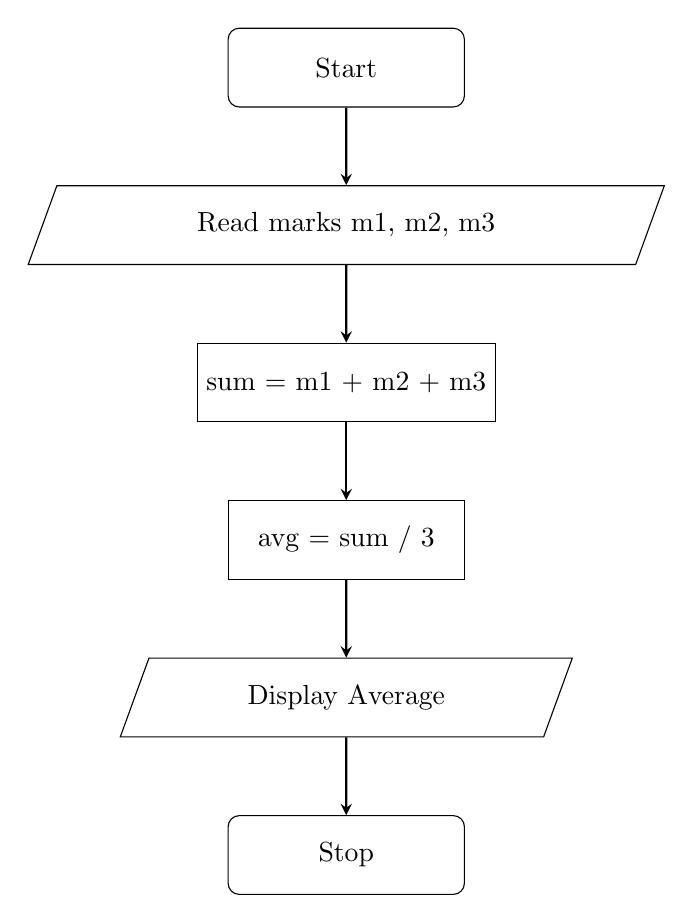
\begin{tikzpicture}[node distance=2cm]
\node (start) [startstop] {Start};
\node (input) [inputoutput, below of=start] 
{Read marks m1, m2, m3};
\node (process1) [process, below of=input] 
{sum = m1 + m2 + m3};
\node (process2) [process, below of=process1] 
{avg = sum / 3};
\node (output) [inputoutput, below of=process2] 
{Display Average};
\node (stop) [startstop, below of=output] {Stop};

\draw [arrow] (start) -- (input);
\draw [arrow] (input) -- (process1);
\draw [arrow] (process1) -- (process2);
\draw [arrow] (process2) -- (output);
\draw [arrow] (output) -- (stop);

\end{tikzpicture}
\end{center}
}

\newcommand{\flowtwo}{
\begin{center}
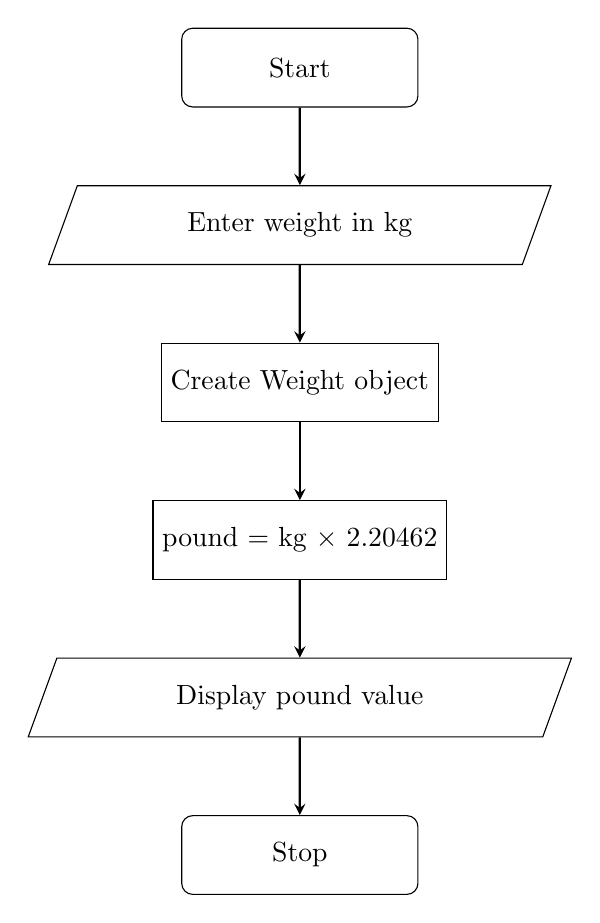
\begin{tikzpicture}[node distance=2cm]

\node (start) [startstop] {Start};

\node (input) [inputoutput, below of=start]
{Enter weight in kg};

\node (process1) [process, below of=input]
{Create Weight object};

\node (process2) [process, below of=process1]
{pound = kg $\times$ 2.20462};

\node (output) [inputoutput, below of=process2]
{Display pound value};

\node (stop) [startstop, below of=output]
{Stop};

\draw [arrow] (start) -- (input);
\draw [arrow] (input) -- (process1);
\draw [arrow] (process1) -- (process2);
\draw [arrow] (process2) -- (output);
\draw [arrow] (output) -- (stop);

\end{tikzpicture}
\end{center}
}

\newcommand{\flowthree}{
\begin{center}
\begin{tikzpicture}[node distance=2cm]

\node (start) [startstop] {Start};

\node (input) [inputoutput, below of=start]
{Enter sides $a, b, c$};

\node (decision) [decision, below of=input, yshift=-0.5cm]
{Are $a,b,c > 0$?};

\node (process1) [process, below of=decision, yshift=-0.7cm]
{Create Prism Object};

\node (process2) [process, below of=process1]
{Surface Area = $2(ab+bc+ac)$};

\node (output1) [inputoutput, below of=process2]
{Display Surface Area};

\node (error) [inputoutput, right of=decision, xshift=6cm]
{Display Error Message};

\node (stop) [startstop, below of=output1]
{Stop};

\draw [arrow] (start) -- (input);
\draw [arrow] (input) -- (decision);

\draw [arrow] (decision) -- node[left]{Yes} (process1);
\draw [arrow] (process1) -- (process2);
\draw [arrow] (process2) -- (output1);
\draw [arrow] (output1) -- (stop);

\draw [arrow] (decision) -- node[above]{No} (error);
\draw [arrow] (error) |- (stop);

\end{tikzpicture}
\end{center}
}

\newcommand{\flowfour}{
\begin{center}
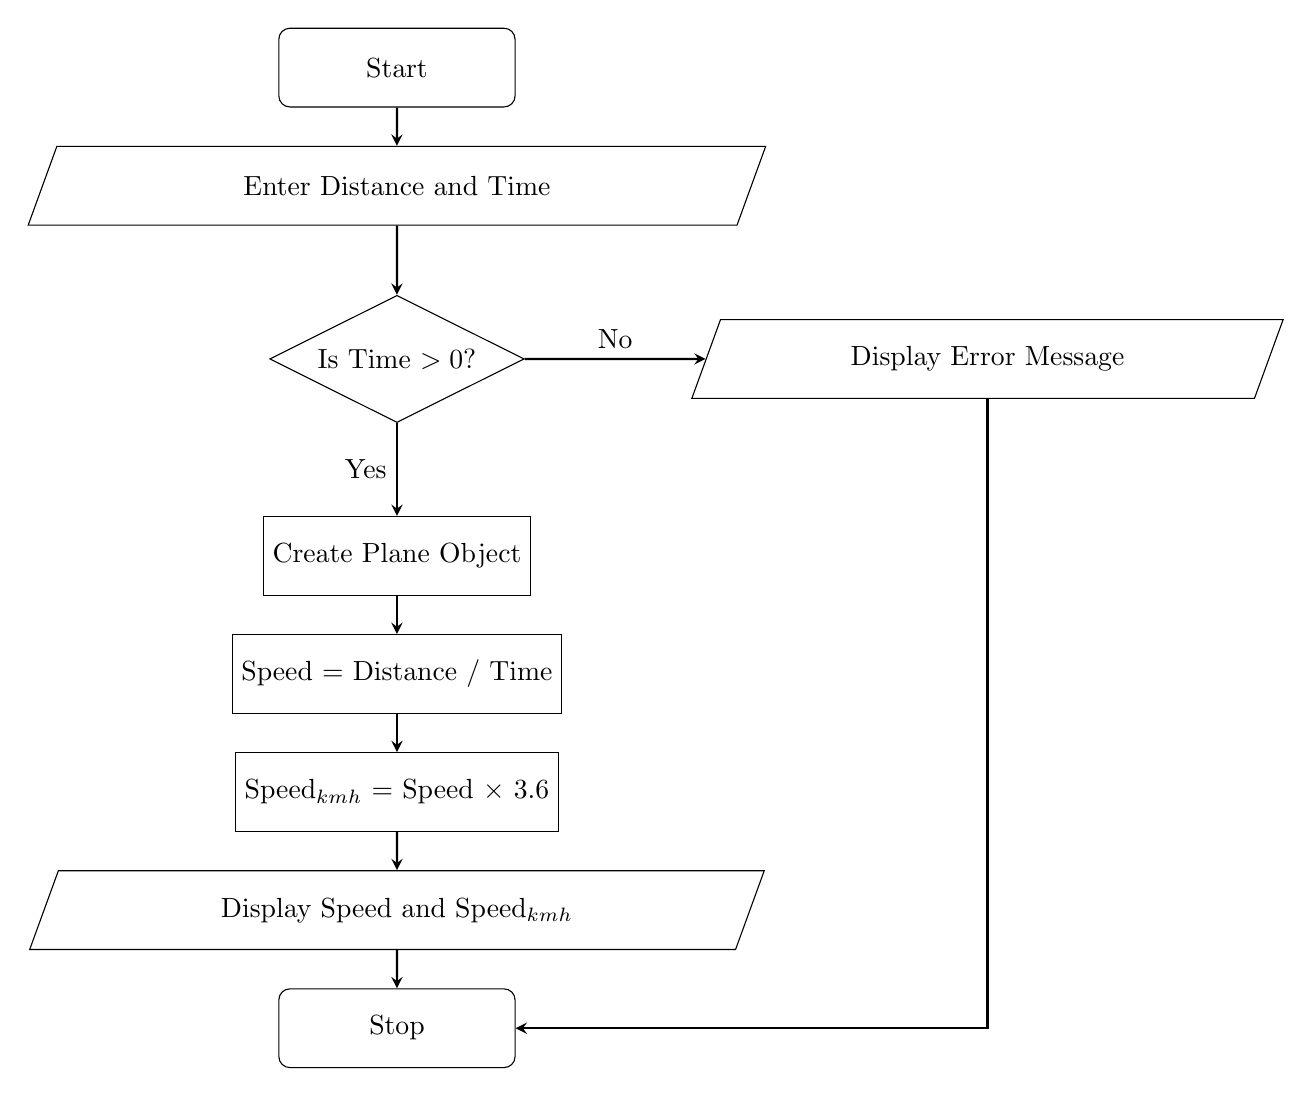
\begin{tikzpicture}[node distance=1.5cm]

\node (start) [startstop] {Start};

\node (input) [inputoutput, below of=start]
{Enter Distance and Time};

\node (decision) [decision, below of=input, yshift=-0.7cm]
{Is Time $> 0$?};

\node (process1) [process, below of=decision, yshift=-1cm]
{Create Plane Object};

\node (process2) [process, below of=process1]
{Speed = Distance / Time};

\node (process3) [process, below of=process2]
{Speed$_{kmh}$ = Speed $\times$ 3.6};

\node (output) [inputoutput, below of=process3]
{Display Speed and Speed$_{kmh}$};

\node (error) [inputoutput, right of=decision, xshift=6cm]
{Display Error Message};

\node (stop) [startstop, below of=output]
{Stop};

\draw [arrow] (start) -- (input);
\draw [arrow] (input) -- (decision);

\draw [arrow] (decision) -- node[left]{Yes} (process1);
\draw [arrow] (process1) -- (process2);
\draw [arrow] (process2) -- (process3);
\draw [arrow] (process3) -- (output);
\draw [arrow] (output) -- (stop);

\draw [arrow] (decision) -- node[above]{No} (error);
\draw [arrow] (error) |- (stop);

\end{tikzpicture}
\end{center}
}

\newcommand{\flowfive}{
\begin{center}
\begin{tikzpicture}[node distance=1.7cm]

\node (start) [startstop] {Start};

\node (input) [inputoutput, below of=start]
{Enter $a$, $b$, $c$, and Flow Rate};

\node (decision) [decision, below of=input, yshift=-1.5cm]
{Are $a,b,c,$ Flow Rate $>0$?};

\node (process1) [process, below of=decision, yshift=-1.7cm]
{Create Pool Object};

\node (process2) [process, below of=process1]
{Volume = $a \times b \times c$};

\node (process3) [process, below of=process2]
{Create Pump Object};

\node (process4) [process, below of=process3]
{Time = Volume / Flow Rate};

\node (process5) [process, below of=process4]
{Create Hour Object};

\node (process6) [process, below of=process5]
{Convert Time to H:M:S};

\node (output) [inputoutput, below of=process6]
{Display Emptying Time};

\node (error) [inputoutput, right of=decision, xshift=7cm]
{Display Error Message};

\node (stop) [startstop, below of=output]
{Stop};

\draw [arrow] (start) -- (input);
\draw [arrow] (input) -- (decision);

\draw [arrow] (decision) -- node[left]{Yes} (process1);
\draw [arrow] (process1) -- (process2);
\draw [arrow] (process2) -- (process3);
\draw [arrow] (process3) -- (process4);
\draw [arrow] (process4) -- (process5);
\draw [arrow] (process5) -- (process6);
\draw [arrow] (process6) -- (output);
\draw [arrow] (output) -- (stop);

\draw [arrow] (decision) -- node[above]{No} (error);
\draw [arrow] (error) |- (stop);

\end{tikzpicture}
\end{center}
}

\newcommand{\flowsix}{
\begin{center}
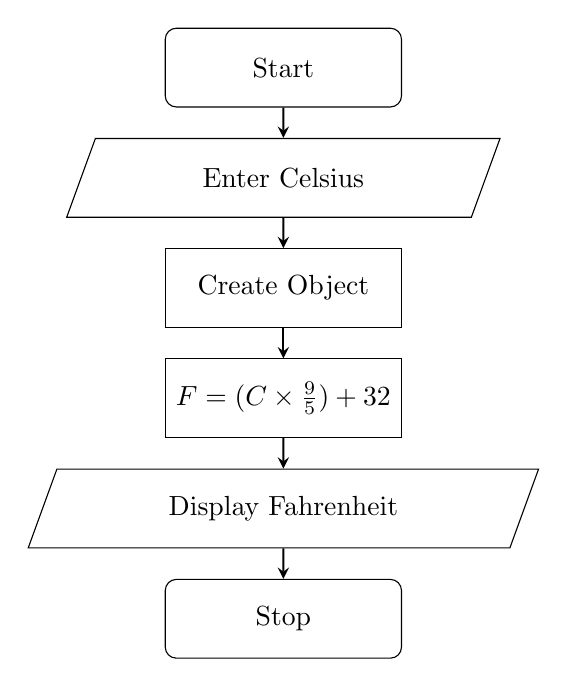
\begin{tikzpicture}[node distance=1.4cm]

\node (start) [startstop] {Start};

\node (input) [inputoutput, below of=start]
{Enter Celsius};

\node (process1) [process, below of=input]
{Create Object};

\node (process2) [process, below of=process1]
{$F=(C \times \frac{9}{5})+32$};

\node (output) [inputoutput, below of=process2]
{Display Fahrenheit};

\node (stop) [startstop, below of=output]
{Stop};

\draw [arrow] (start) -- (input);
\draw [arrow] (input) -- (process1);
\draw [arrow] (process1) -- (process2);
\draw [arrow] (process2) -- (output);
\draw [arrow] (output) -- (stop);

\end{tikzpicture}
\end{center}
}

\newcommand{\flowseven}{
\begin{center}
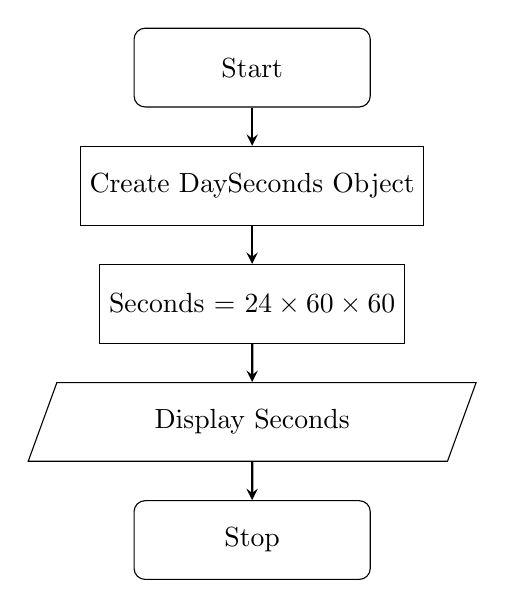
\begin{tikzpicture}[node distance=1.5cm]

\node (start) [startstop] {Start};

\node (process1) [process, below of=start]
{Create DaySeconds Object};

\node (process2) [process, below of=process1]
{Seconds = $24 \times 60 \times 60$};

\node (output) [inputoutput, below of=process2]
{Display Seconds};

\node (stop) [startstop, below of=output]
{Stop};

\draw [arrow] (start) -- (process1);
\draw [arrow] (process1) -- (process2);
\draw [arrow] (process2) -- (output);
\draw [arrow] (output) -- (stop);

\end{tikzpicture}
\end{center}
}

\newcommand{\floweight}{
\begin{center}
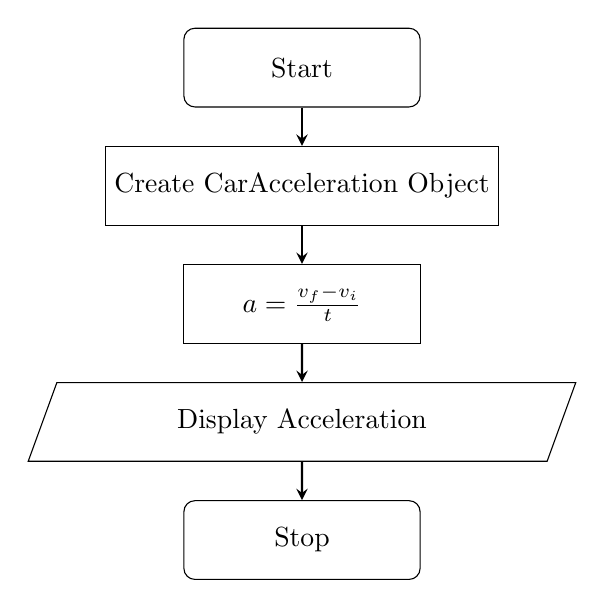
\begin{tikzpicture}[node distance=1.5cm]

\node (start) [startstop] {Start};

\node (process1) [process, below of=start]
{Create CarAcceleration Object};

\node (process2) [process, below of=process1]
{$a=\frac{v_f-v_i}{t}$};

\node (output) [inputoutput, below of=process2]
{Display Acceleration};

\node (stop) [startstop, below of=output]
{Stop};

\draw [arrow] (start) -- (process1);
\draw [arrow] (process1) -- (process2);
\draw [arrow] (process2) -- (output);
\draw [arrow] (output) -- (stop);

\end{tikzpicture}
\end{center}
}

\newcommand{\flownine}{
\begin{center}
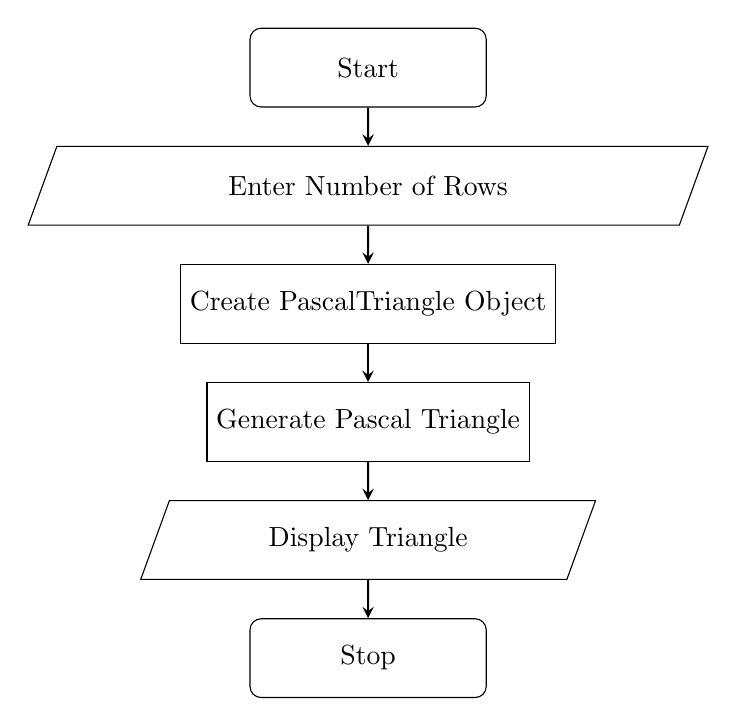
\begin{tikzpicture}[node distance=1.5cm]

\node (start) [startstop] {Start};

\node (input) [inputoutput, below of=start]
{Enter Number of Rows};

\node (process1) [process, below of=input]
{Create PascalTriangle Object};

\node (process2) [process, below of=process1]
{Generate Pascal Triangle};

\node (output) [inputoutput, below of=process2]
{Display Triangle};

\node (stop) [startstop, below of=output]
{Stop};

\draw [arrow] (start) -- (input);
\draw [arrow] (input) -- (process1);
\draw [arrow] (process1) -- (process2);
\draw [arrow] (process2) -- (output);
\draw [arrow] (output) -- (stop);

\end{tikzpicture}
\end{center}
}

\newcommand{\flowten}{
\begin{center}
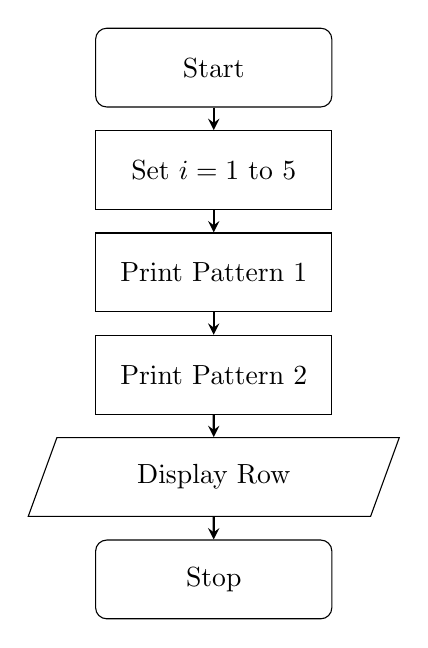
\begin{tikzpicture}[node distance=1.3cm]

\node (start) [startstop] {Start};

\node (process1) [process, below of=start]
{Set $i=1$ to $5$};

\node (process2) [process, below of=process1]
{Print Pattern 1};

\node (process3) [process, below of=process2]
{Print Pattern 2};

\node (output) [inputoutput, below of=process3]
{Display Row};

\node (stop) [startstop, below of=output]
{Stop};

\draw [arrow] (start) -- (process1);
\draw [arrow] (process1) -- (process2);
\draw [arrow] (process2) -- (process3);
\draw [arrow] (process3) -- (output);
\draw [arrow] (output) -- (stop);

\end{tikzpicture}
\end{center}
}

\newcommand{\floweleven}{
\begin{center}
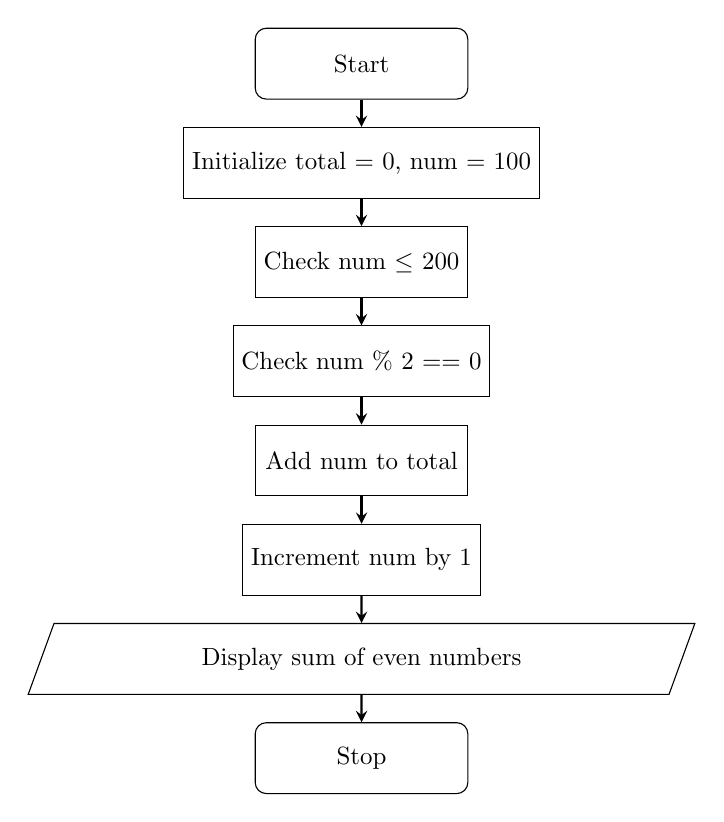
\begin{tikzpicture}[node distance=1.4cm, scale=0.9, transform shape]

\node (start) [startstop] {Start};

\node (init) [process, below of=start] 
{Initialize total = 0, num = 100};

\node (check) [process, below of=init] 
{Check num $\leq$ 200};

\node (even) [process, below of=check] 
{Check num \% 2 == 0};

\node (add) [process, below of=even] 
{Add num to total};

\node (inc) [process, below of=add] 
{Increment num by 1};

\node (output) [inputoutput, below of=inc] 
{Display sum of even numbers};

\node (stop) [startstop, below of=output] {Stop};

\draw [arrow] (start) -- (init);
\draw [arrow] (init) -- (check);
\draw [arrow] (check) -- (even);
\draw [arrow] (even) -- (add);
\draw [arrow] (add) -- (inc);
\draw [arrow] (inc) -- (output);
\draw [arrow] (output) -- (stop);

\end{tikzpicture}
\end{center}
}

\newcommand{\flowtwelve}{
\begin{center}
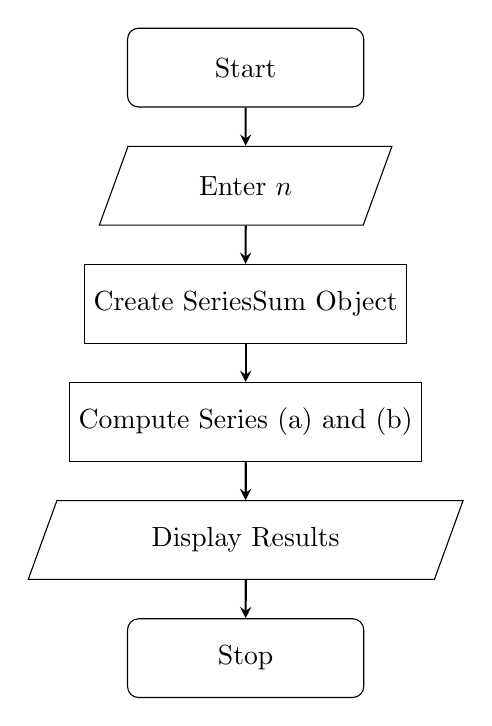
\begin{tikzpicture}[node distance=1.5cm]

\node (start) [startstop] {Start};

\node (input) [inputoutput, below of=start]
{Enter $n$};

\node (process1) [process, below of=input]
{Create SeriesSum Object};

\node (process2) [process, below of=process1]
{Compute Series (a) and (b)};

\node (output) [inputoutput, below of=process2]
{Display Results};

\node (stop) [startstop, below of=output]
{Stop};

\draw [arrow] (start) -- (input);
\draw [arrow] (input) -- (process1);
\draw [arrow] (process1) -- (process2);
\draw [arrow] (process2) -- (output);
\draw [arrow] (output) -- (stop);

\end{tikzpicture}
\end{center}
}

\newcommand{\flowthirteen}{
\begin{center}
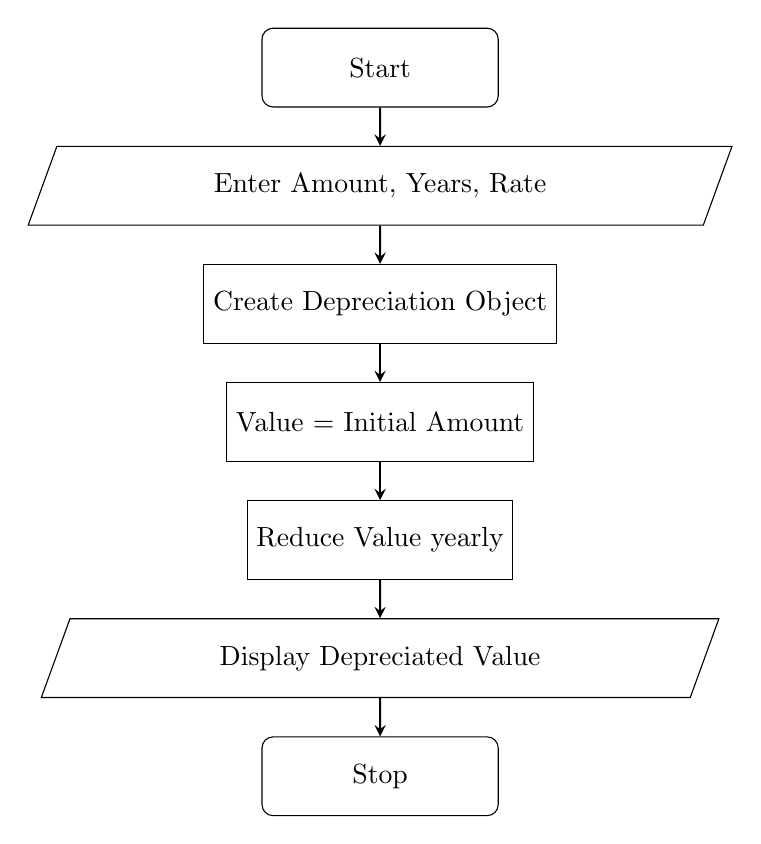
\begin{tikzpicture}[node distance=1.5cm]

\node (start) [startstop] {Start};

\node (input) [inputoutput, below of=start]
{Enter Amount, Years, Rate};

\node (process1) [process, below of=input]
{Create Depreciation Object};

\node (process2) [process, below of=process1]
{Value = Initial Amount};

\node (process3) [process, below of=process2]
{Reduce Value yearly};

\node (output) [inputoutput, below of=process3]
{Display Depreciated Value};

\node (stop) [startstop, below of=output]
{Stop};

\draw [arrow] (start) -- (input);
\draw [arrow] (input) -- (process1);
\draw [arrow] (process1) -- (process2);
\draw [arrow] (process2) -- (process3);
\draw [arrow] (process3) -- (output);
\draw [arrow] (output) -- (stop);

\end{tikzpicture}
\end{center}
}

\newcommand{\flowfourteen}{
\begin{center}
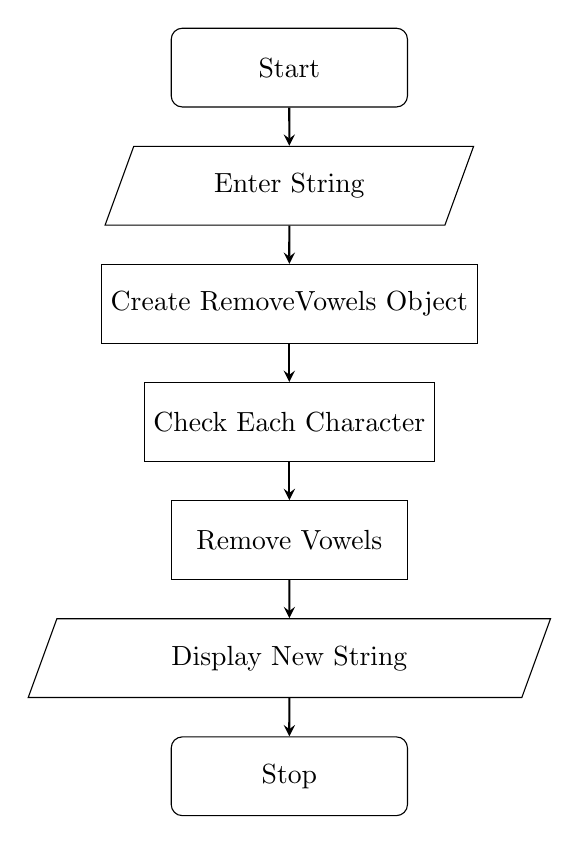
\begin{tikzpicture}[node distance=1.5cm]

\node (start) [startstop] {Start};

\node (input) [inputoutput, below of=start]
{Enter String};

\node (process1) [process, below of=input]
{Create RemoveVowels Object};

\node (process2) [process, below of=process1]
{Check Each Character};

\node (process3) [process, below of=process2]
{Remove Vowels};

\node (output) [inputoutput, below of=process3]
{Display New String};

\node (stop) [startstop, below of=output]
{Stop};

\draw [arrow] (start) -- (input);
\draw [arrow] (input) -- (process1);
\draw [arrow] (process1) -- (process2);
\draw [arrow] (process2) -- (process3);
\draw [arrow] (process3) -- (output);
\draw [arrow] (output) -- (stop);

\end{tikzpicture}
\end{center}
}

\newcommand{\flowfifteen}{
\begin{center}
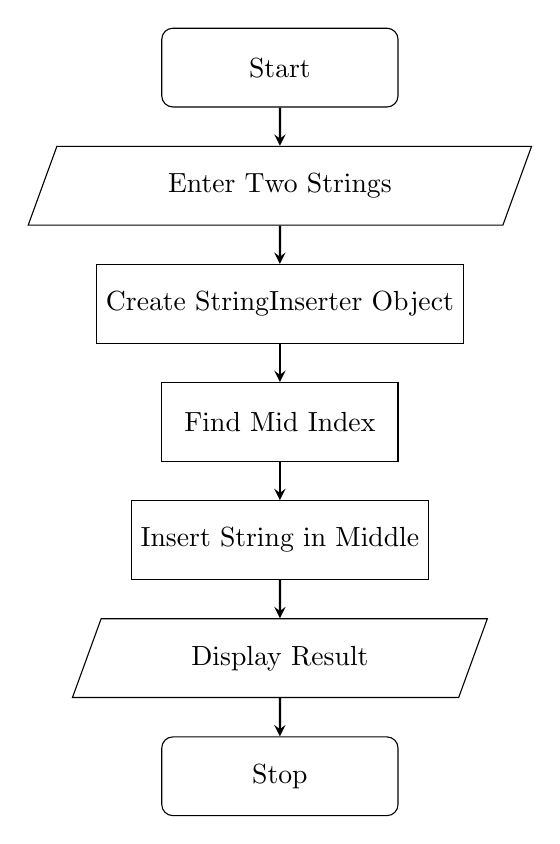
\begin{tikzpicture}[node distance=1.5cm]

\node (start) [startstop] {Start};

\node (input) [inputoutput, below of=start]
{Enter Two Strings};

\node (process1) [process, below of=input]
{Create StringInserter Object};

\node (process2) [process, below of=process1]
{Find Mid Index};

\node (process3) [process, below of=process2]
{Insert String in Middle};

\node (output) [inputoutput, below of=process3]
{Display Result};

\node (stop) [startstop, below of=output]
{Stop};

\draw [arrow] (start) -- (input);
\draw [arrow] (input) -- (process1);
\draw [arrow] (process1) -- (process2);
\draw [arrow] (process2) -- (process3);
\draw [arrow] (process3) -- (output);
\draw [arrow] (output) -- (stop);

\end{tikzpicture}
\end{center}
}

\newcommand{\flowsixteen}{
\begin{center}
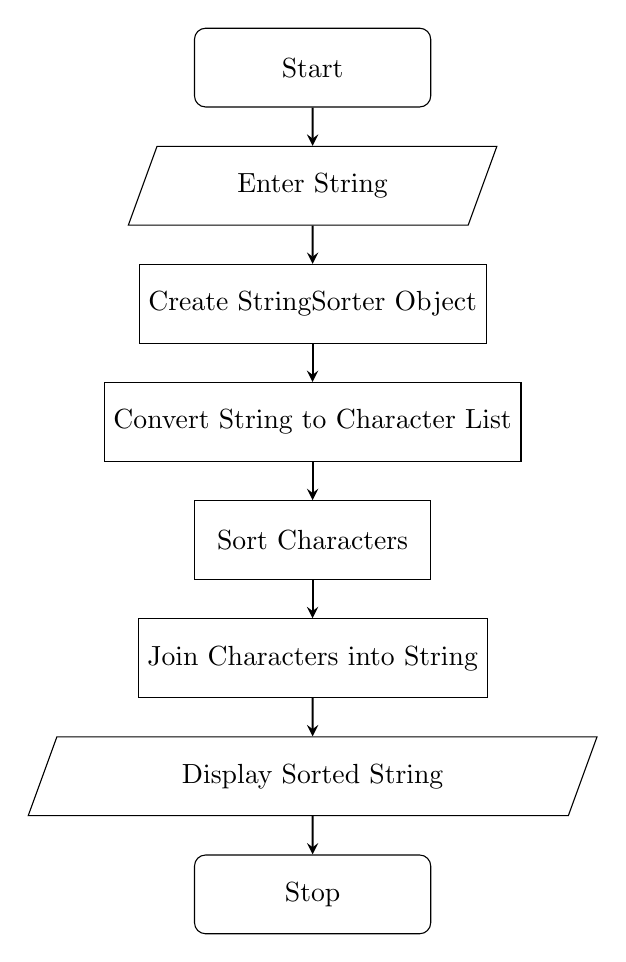
\begin{tikzpicture}[node distance=1.5cm]

\node (start) [startstop] {Start};

\node (input) [inputoutput, below of=start]
{Enter String};

\node (process1) [process, below of=input]
{Create StringSorter Object};

\node (process2) [process, below of=process1]
{Convert String to Character List};

\node (process3) [process, below of=process2]
{Sort Characters};

\node (process4) [process, below of=process3]
{Join Characters into String};

\node (output) [inputoutput, below of=process4]
{Display Sorted String};

\node (stop) [startstop, below of=output]
{Stop};

\draw [arrow] (start) -- (input);
\draw [arrow] (input) -- (process1);
\draw [arrow] (process1) -- (process2);
\draw [arrow] (process2) -- (process3);
\draw [arrow] (process3) -- (process4);
\draw [arrow] (process4) -- (output);
\draw [arrow] (output) -- (stop);

\end{tikzpicture}
\end{center}
}

\newcommand{\flowseventeen}{
\begin{center}
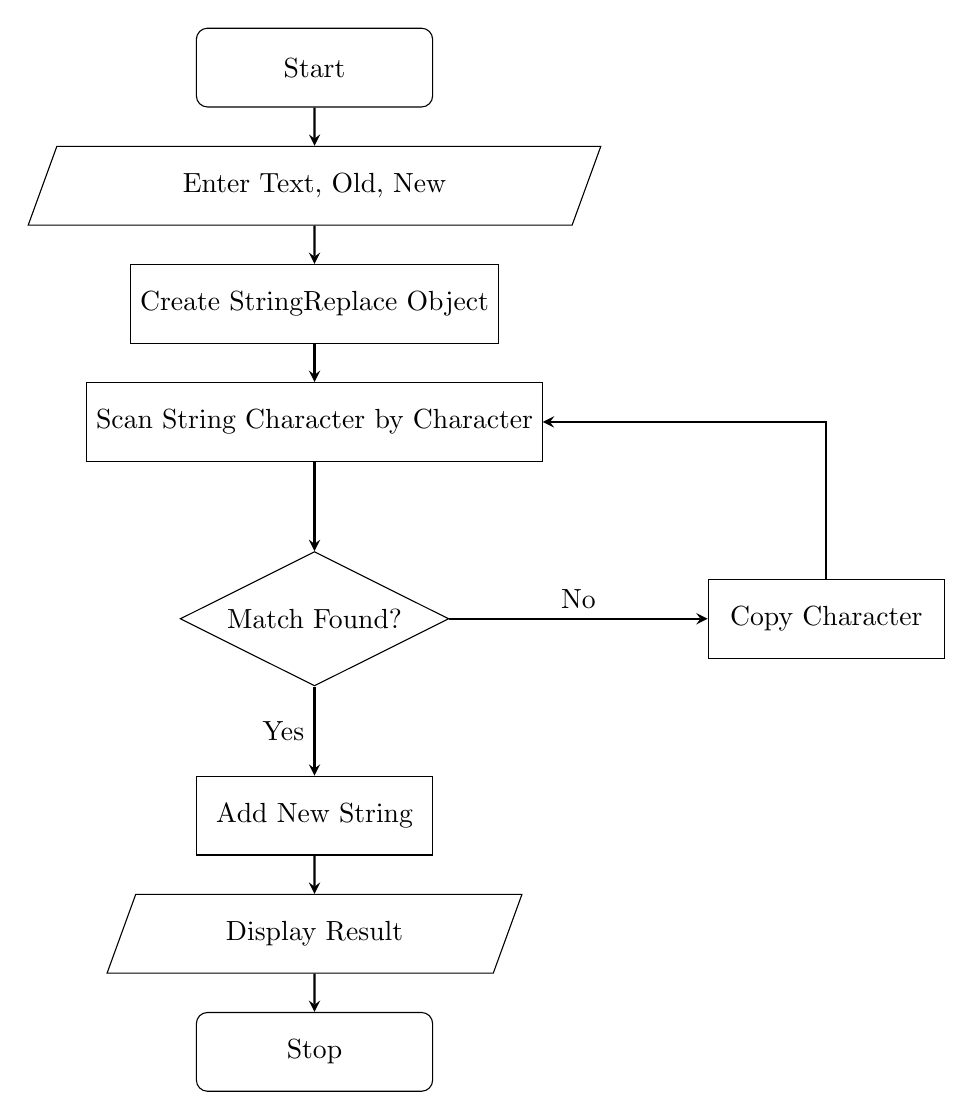
\begin{tikzpicture}[node distance=1.5cm]

\node (start) [startstop] {Start};

\node (input) [inputoutput, below of=start]
{Enter Text, Old, New};

\node (process1) [process, below of=input]
{Create StringReplace Object};

\node (process2) [process, below of=process1]
{Scan String Character by Character};

\node (decision) [decision, below of=process2, yshift=-1cm]
{Match Found?};

\node (replace) [process, below of=decision, yshift=-1cm]
{Add New String};

\node (copy) [process, right of=decision, xshift=5cm]
{Copy Character};

\node (output) [inputoutput, below of=replace]
{Display Result};

\node (stop) [startstop, below of=output]
{Stop};

\draw [arrow] (start) -- (input);
\draw [arrow] (input) -- (process1);
\draw [arrow] (process1) -- (process2);

\draw [arrow] (process2) -- (decision);

\draw [arrow] (decision) -- node[left]{Yes} (replace);
\draw [arrow] (decision) -- node[above]{No} (copy);

\draw [arrow] (copy) |- (process2);

\draw [arrow] (replace) -- (output);
\draw [arrow] (output) -- (stop);

\end{tikzpicture}
\end{center}
}

\newcommand{\floweighteen}{
\begin{center}
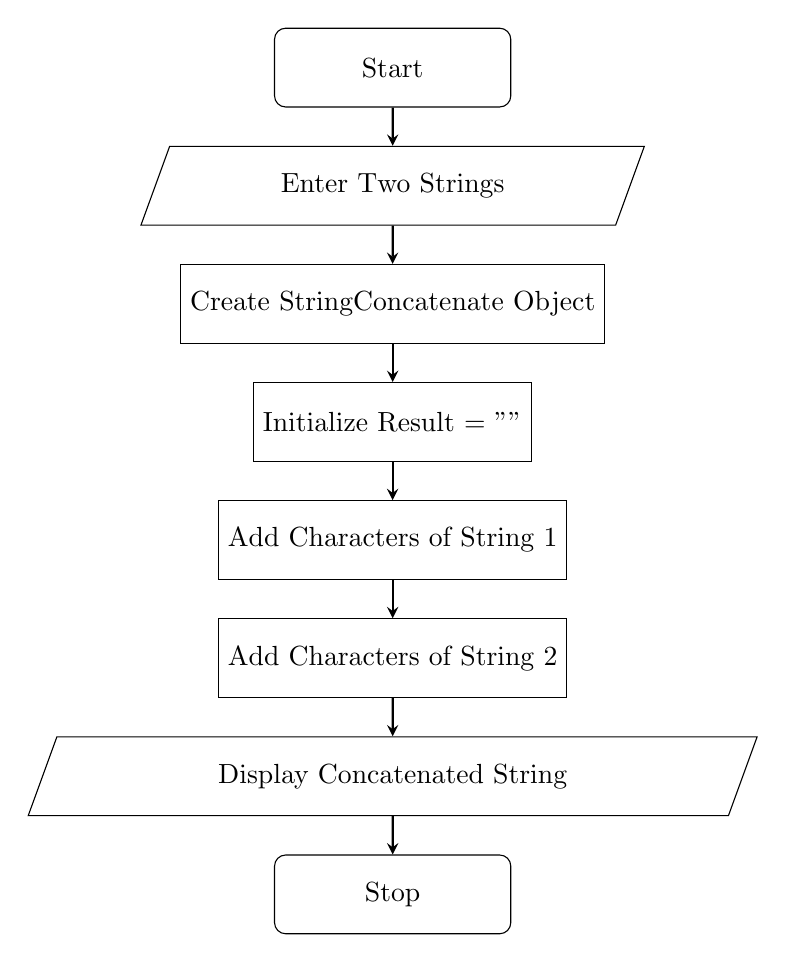
\begin{tikzpicture}[node distance=1.5cm]

\node (start) [startstop] {Start};

\node (input) [inputoutput, below of=start]
{Enter Two Strings};

\node (process1) [process, below of=input]
{Create StringConcatenate Object};

\node (process2) [process, below of=process1]
{Initialize Result = ""};

\node (process3) [process, below of=process2]
{Add Characters of String 1};

\node (process4) [process, below of=process3]
{Add Characters of String 2};

\node (output) [inputoutput, below of=process4]
{Display Concatenated String};

\node (stop) [startstop, below of=output]
{Stop};

\draw [arrow] (start) -- (input);
\draw [arrow] (input) -- (process1);
\draw [arrow] (process1) -- (process2);
\draw [arrow] (process2) -- (process3);
\draw [arrow] (process3) -- (process4);
\draw [arrow] (process4) -- (output);
\draw [arrow] (output) -- (stop);

\end{tikzpicture}
\end{center}
}

\newcommand{\flownineteen}{
\begin{center}
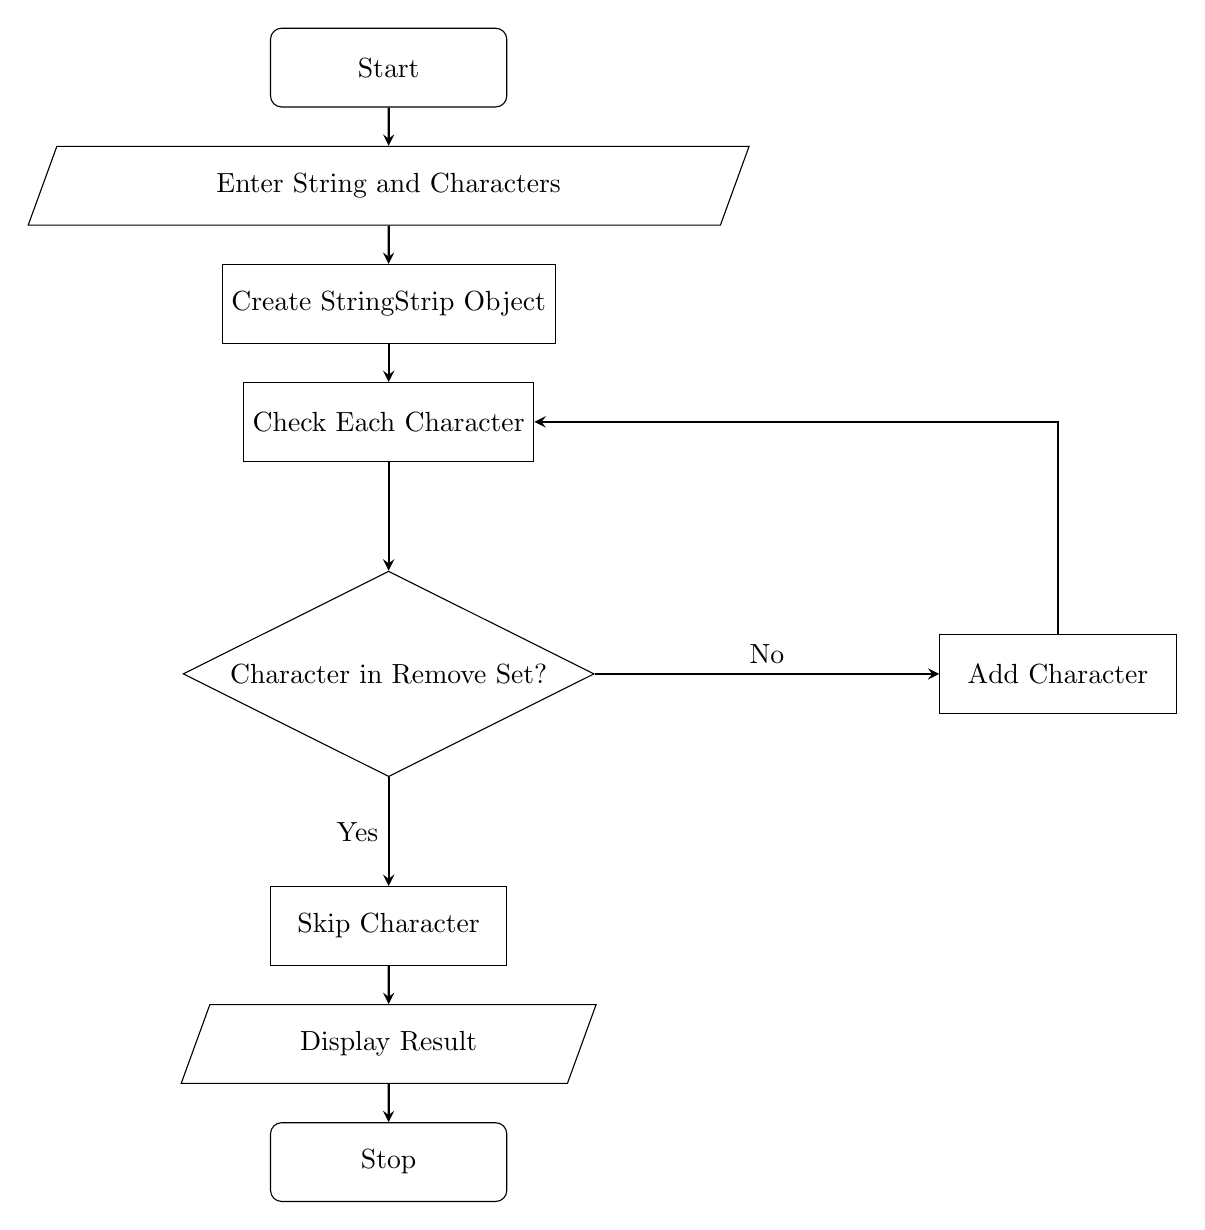
\begin{tikzpicture}[node distance=1.5cm]

\node (start) [startstop] {Start};

\node (input) [inputoutput, below of=start]
{Enter String and Characters};

\node (process1) [process, below of=input]
{Create StringStrip Object};

\node (process2) [process, below of=process1]
{Check Each Character};

\node (decision) [decision, below of=process2, yshift=-1.7cm]
{Character in Remove Set?};

\node (remove) [process, below of=decision, yshift=-1.7cm]
{Skip Character};

\node (keep) [process, right of=decision, xshift=7cm]
{Add Character};

\node (output) [inputoutput, below of=remove]
{Display Result};

\node (stop) [startstop, below of=output]
{Stop};

\draw [arrow] (start) -- (input);
\draw [arrow] (input) -- (process1);
\draw [arrow] (process1) -- (process2);
\draw [arrow] (process2) -- (decision);

\draw [arrow] (decision) -- node[left]{Yes} (remove);
\draw [arrow] (decision) -- node[above]{No} (keep);

\draw [arrow] (keep) |- (process2);
\draw [arrow] (remove) -- (output);
\draw [arrow] (output) -- (stop);

\end{tikzpicture}
\end{center}
}

\newcommand{\flowtwenty}{
\begin{center}
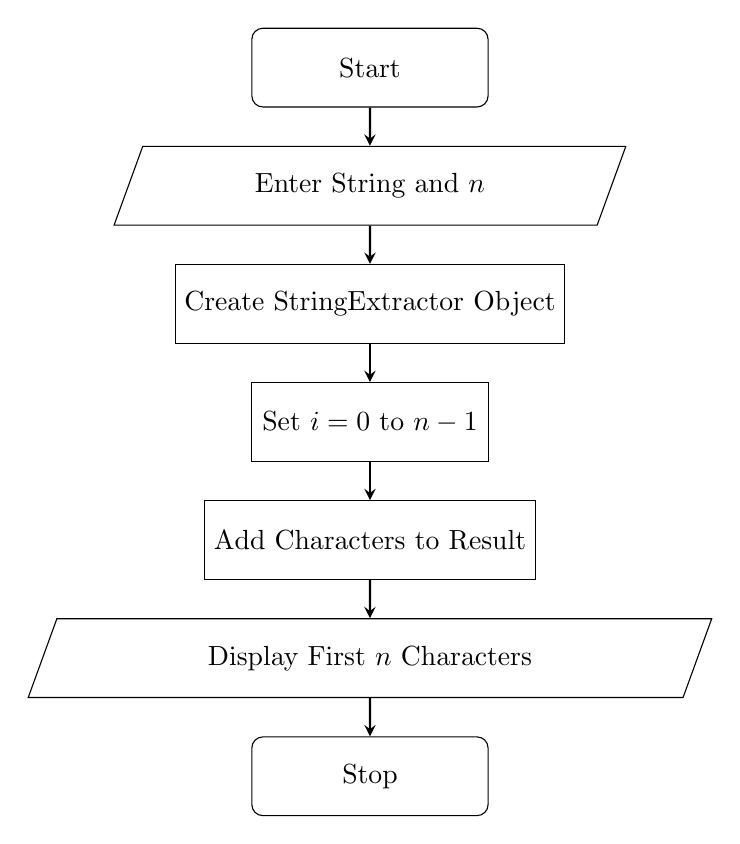
\begin{tikzpicture}[node distance=1.5cm]

\node (start) [startstop] {Start};

\node (input) [inputoutput, below of=start]
{Enter String and $n$};

\node (process1) [process, below of=input]
{Create StringExtractor Object};

\node (process2) [process, below of=process1]
{Set $i=0$ to $n-1$};

\node (process3) [process, below of=process2]
{Add Characters to Result};

\node (output) [inputoutput, below of=process3]
{Display First $n$ Characters};

\node (stop) [startstop, below of=output]
{Stop};

\draw [arrow] (start) -- (input);
\draw [arrow] (input) -- (process1);
\draw [arrow] (process1) -- (process2);
\draw [arrow] (process2) -- (process3);
\draw [arrow] (process3) -- (output);
\draw [arrow] (output) -- (stop);

\end{tikzpicture}
\end{center}
}

\newcommand{\flowtwentyone}{
\begin{center}
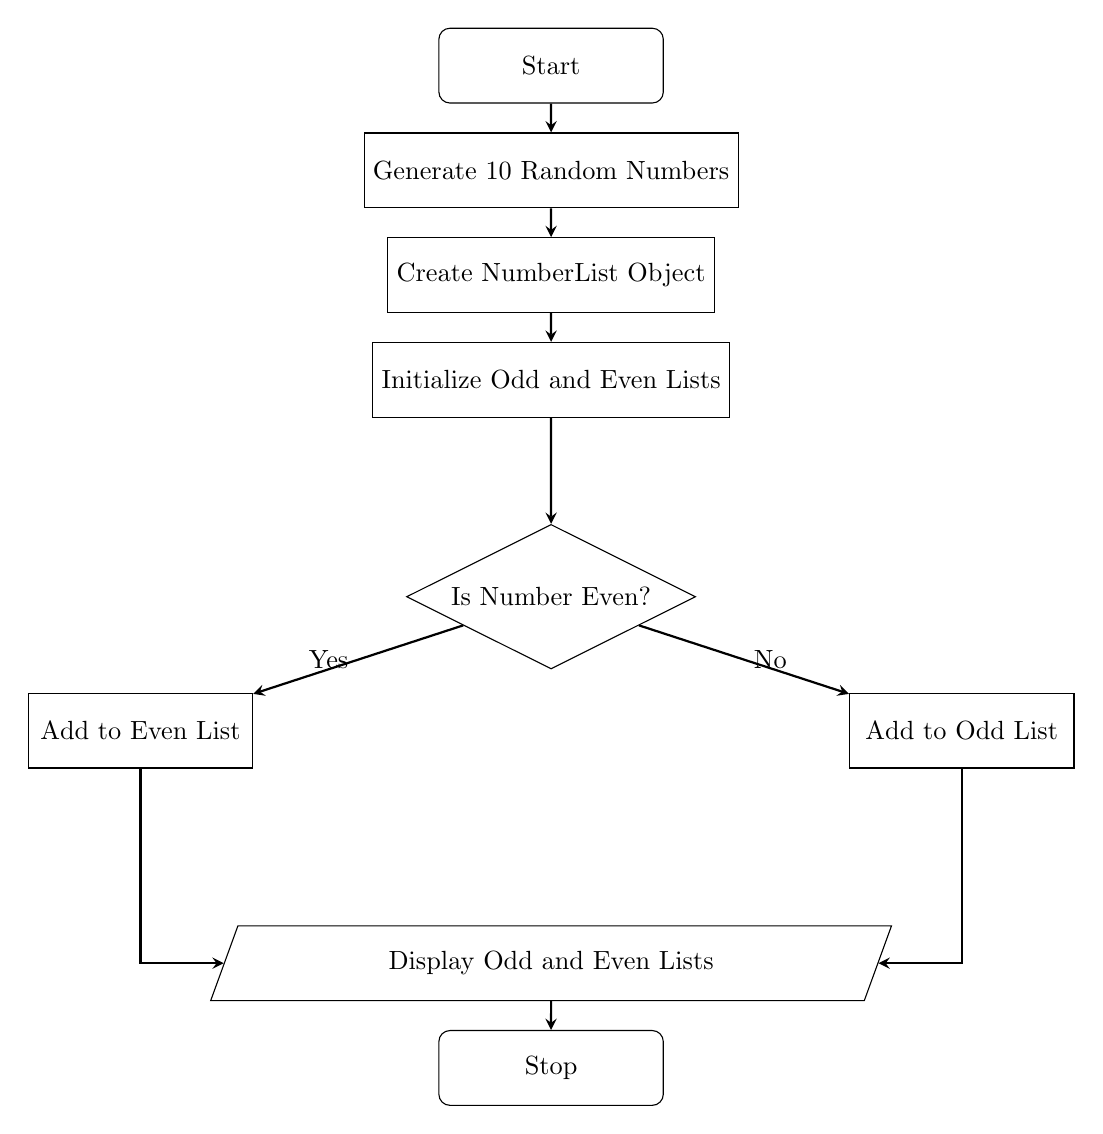
\begin{tikzpicture}[node distance=1.4cm, scale=0.95, transform shape]

\node (start) [startstop] {Start};

\node (init) [process, below of=start]
{Generate 10 Random Numbers};

\node (obj) [process, below of=init]
{Create NumberList Object};

\node (lists) [process, below of=obj]
{Initialize Odd and Even Lists};

\node (decision) [decision, below of=lists, yshift=-1.5cm]
{Is Number Even?};

\node (even) [process, below left of=decision, xshift=-4.5cm, yshift=-0.8cm]
{Add to Even List};

\node (odd) [process, below right of=decision, xshift=4.5cm, yshift=-0.8cm]
{Add to Odd List};

\node (display) [inputoutput, below of=decision, yshift=-3.5cm]
{Display Odd and Even Lists};

\node (stop) [startstop, below of=display]
{Stop};

\draw [arrow] (start) -- (init);
\draw [arrow] (init) -- (obj);
\draw [arrow] (obj) -- (lists);
\draw [arrow] (lists) -- (decision);

\draw [arrow] (decision) -- node[left]{Yes} (even);
\draw [arrow] (decision) -- node[right]{No} (odd);

\draw [arrow] (even) |- (display);
\draw [arrow] (odd) |- (display);

\draw [arrow] (display) -- (stop);

\end{tikzpicture}
\end{center}
}

\newcommand{\flowtwentytwo}{
\begin{center}
\begin{tikzpicture}[node distance=1.5cm, scale=0.95, transform shape]

\node (start) [startstop] {Start};

\node (input) [inputoutput, below of=start]
{Input Array};

\node (init) [process, below of=input]
{i = 1};

\node (check1) [decision, below of=init, yshift=-0.3cm]
{i $<$ n ?};

% Added align=center here
\node (setkey) [process, below of=check1, yshift=-0.8cm, align=center]
{key = arr[i]\\
j = i - 1};

% Added align=center here
\node (check2) [decision, below of=setkey, yshift=-1.8cm, align=center]
{j $\geq$ 0 and\\
arr[j] $>$ key ?};

% Added align=center here
\node (shift) [process, right of=check2, xshift=4cm, align=center, xshift=3cm]
{arr[j+1] = arr[j]\\
j = j - 1};

\node (insert) [process, below of=check2, yshift=-1.8cm]
{arr[j+1] = key};

\node (inc) [process, below of=insert]
{i = i + 1};

\node (output) [inputoutput, below of=inc]
{Display Sorted Array};

\node (stop) [startstop, below of=output]
{Stop};

\draw [arrow] (start) -- (input);
\draw [arrow] (input) -- (init);
\draw [arrow] (init) -- (check1);

\draw [arrow] (check1) -- node[right]{Yes} (setkey);
\draw [arrow] (setkey) -- (check2);

\draw [arrow] (check2) -- node[above]{Yes} (shift);

\draw [arrow] (check2) -- node[left]{No} (insert);

\draw [arrow] (insert) -- (inc);
\draw [arrow] (inc.east) -- ++(4,0)
node[midway,above]
|- (shift.west);

\draw [arrow] (check1.east) -- ++(2,0)
node[midway,above]{No}
|- (output.east);

\draw [arrow] (output) -- (stop);

\end{tikzpicture}
\end{center}
}

\newcommand{\flowtwentythree}{
\begin{center}
\begin{tikzpicture}[node distance=2cm, scale=0.95, transform shape]

\node (start) [startstop] {Start};

\node (input) [inputoutput, below of=start, align=center]
{Input Sorted Array\\and Key};

\node (init) [process, below of=input, align=center]
{low = 0\\
high = n - 1};

\node (check1) [decision, below of=init, yshift=-0.5cm]
{low $\leq$ high ?};

\node (mid) [process, below of=check1, yshift=-1cm]
{mid = (low + high)/2};

\node (check2) [decision, below of=mid, yshift=-0.8cm]
{arr[mid] = key ?};

\node (found) [inputoutput, below of=check2, yshift=-2cm, align=center]
{Display\\Element Found};

\node (check3) [decision, right of=check2, xshift=6cm, align=center]
{arr[mid] $<$ key ?};

\node (lowup) [process, below of=check3, yshift=-2cm]
{low = mid + 1};

\node (highup) [process, above of=check3, yshift=2cm]
{high = mid - 1};

\node (notfound) [inputoutput, below of=found, yshift=-0.5cm, align=center, xshift=4cm]
{Display\\Element Not Found};

\node (stop) [startstop, below of=notfound, xshift=-4cm]
{Stop};

% Arrows
\draw [arrow] (start) -- (input);
\draw [arrow] (input) -- (init);
\draw [arrow] (init) -- (check1);

\draw [arrow] (check1) -- node[right]{Yes} (mid);
\draw [arrow] (mid) -- (check2);

\draw [arrow] (check2) -- node[left]{Yes} (found);

\draw [arrow] (check2) -- node[above]{No} (check3);

\draw [arrow] (check3) -- node[right]{Yes} (lowup);
\draw [arrow] (lowup.east) -- ++(4,0)
node[midway,above]{No}
|- (check1.east);

\draw [arrow] (check3) -- node[right]{No} (highup);
\draw [arrow] (highup) |- (check1);

\draw [arrow] (check1.east) -- ++(9,0)
node[midway,above]{No}
|- (notfound.east);

\draw [arrow] (found) -- (stop);
\draw [arrow] (notfound.south) -- ++(0,0)
node[midway,above]
|- (stop.east);

\end{tikzpicture}
\end{center}
}

\newcommand{\flowtwentyfour}{
\begin{center}
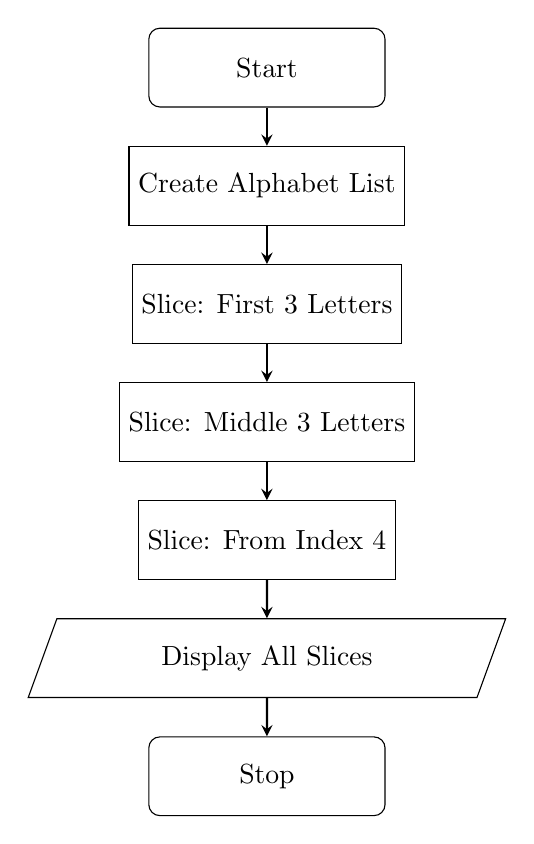
\begin{tikzpicture}[node distance=1.5cm]

\node (start) [startstop] {Start};

\node (process1) [process, below of=start]
{Create Alphabet List};

\node (process2) [process, below of=process1]
{Slice: First 3 Letters};

\node (process3) [process, below of=process2]
{Slice: Middle 3 Letters};

\node (process4) [process, below of=process3]
{Slice: From Index 4};

\node (output) [inputoutput, below of=process4]
{Display All Slices};

\node (stop) [startstop, below of=output]
{Stop};

\draw [arrow] (start) -- (process1);
\draw [arrow] (process1) -- (process2);
\draw [arrow] (process2) -- (process3);
\draw [arrow] (process3) -- (process4);
\draw [arrow] (process4) -- (output);
\draw [arrow] (output) -- (stop);

\end{tikzpicture}
\end{center}
}

\newcommand{\flowtwentyfive}{
\begin{center}
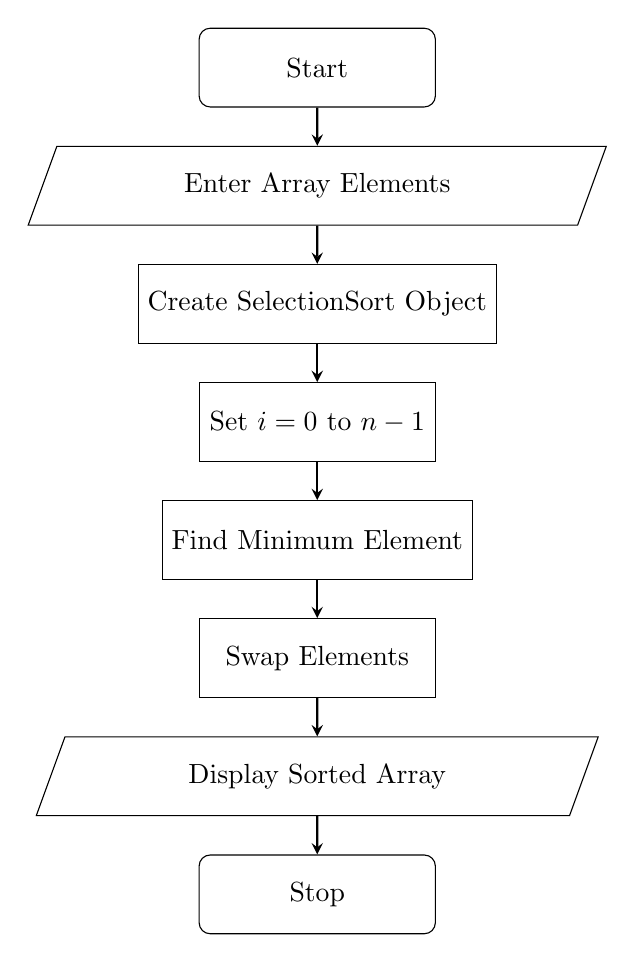
\begin{tikzpicture}[node distance=1.5cm]

\node (start) [startstop] {Start};

\node (input) [inputoutput, below of=start]
{Enter Array Elements};

\node (process1) [process, below of=input]
{Create SelectionSort Object};

\node (process2) [process, below of=process1]
{Set $i=0$ to $n-1$};

\node (process3) [process, below of=process2]
{Find Minimum Element};

\node (process4) [process, below of=process3]
{Swap Elements};

\node (output) [inputoutput, below of=process4]
{Display Sorted Array};

\node (stop) [startstop, below of=output]
{Stop};

\draw [arrow] (start) -- (input);
\draw [arrow] (input) -- (process1);
\draw [arrow] (process1) -- (process2);
\draw [arrow] (process2) -- (process3);
\draw [arrow] (process3) -- (process4);
\draw [arrow] (process4) -- (output);
\draw [arrow] (output) -- (stop);

\end{tikzpicture}
\end{center}
}

\newcommand{\flowtwentysix}{
\begin{center}
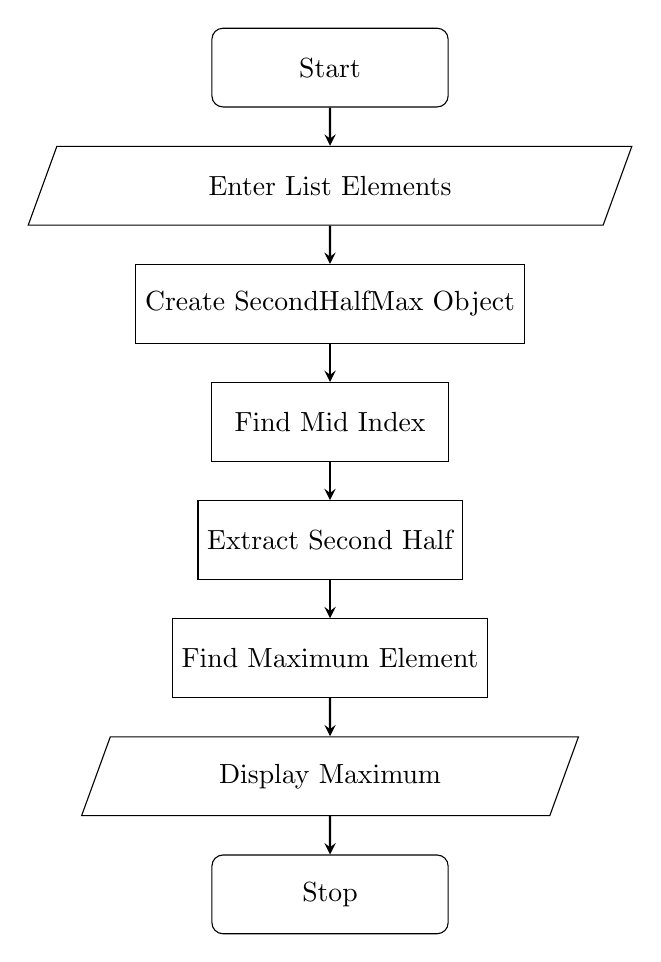
\begin{tikzpicture}[node distance=1.5cm]

\node (start) [startstop] {Start};

\node (input) [inputoutput, below of=start]
{Enter List Elements};

\node (process1) [process, below of=input]
{Create SecondHalfMax Object};

\node (process2) [process, below of=process1]
{Find Mid Index};

\node (process3) [process, below of=process2]
{Extract Second Half};

\node (process4) [process, below of=process3]
{Find Maximum Element};

\node (output) [inputoutput, below of=process4]
{Display Maximum};

\node (stop) [startstop, below of=output]
{Stop};

\draw [arrow] (start) -- (input);
\draw [arrow] (input) -- (process1);
\draw [arrow] (process1) -- (process2);
\draw [arrow] (process2) -- (process3);
\draw [arrow] (process3) -- (process4);
\draw [arrow] (process4) -- (output);
\draw [arrow] (output) -- (stop);

\end{tikzpicture}
\end{center}
}

\newcommand{\flowtwentyseven}{
\begin{center}
\begin{tikzpicture}[node distance=0.5cm]

\node (start) [startstop] {Start};

\node (process1) [process, below of=start, yshift = -1.0cm]
{Create Empty List};

\node (process2) [process, below of=process1, yshift = -1.0cm]
{Loop $i=1$ to $100$};

\node (decision) [decision, below of=process2, yshift=-3cm, align=center]
{Is\\
$i \bmod 5 = 0$\\
or\\
$i \bmod 6 = 0$ ?};


\node (add) [process, below of=decision, yshift = -3cm]
{Add $i$ to List};

\node (skip) [process, right of=decision, xshift=8cm]
{Skip Number};

\node (output) [inputoutput, below of=add, yshift = -1.0cm]
{Display List};

\node (stop) [startstop, below of=output, yshift = -1cm]
{Stop};

\draw [arrow] (start) -- (process1);
\draw [arrow] (process1) -- (process2);
\draw [arrow] (process2) -- (decision);

\draw [arrow] (decision) -- node[left]{Yes} (add);
\draw [arrow] (decision) -- node[above]{No} (skip);

\draw [arrow] (skip) |- (process2);

\draw [arrow] (output) -- (stop);

\end{tikzpicture}
\end{center}
}

\newcommand{\flowtwentyeight}{
\begin{center}
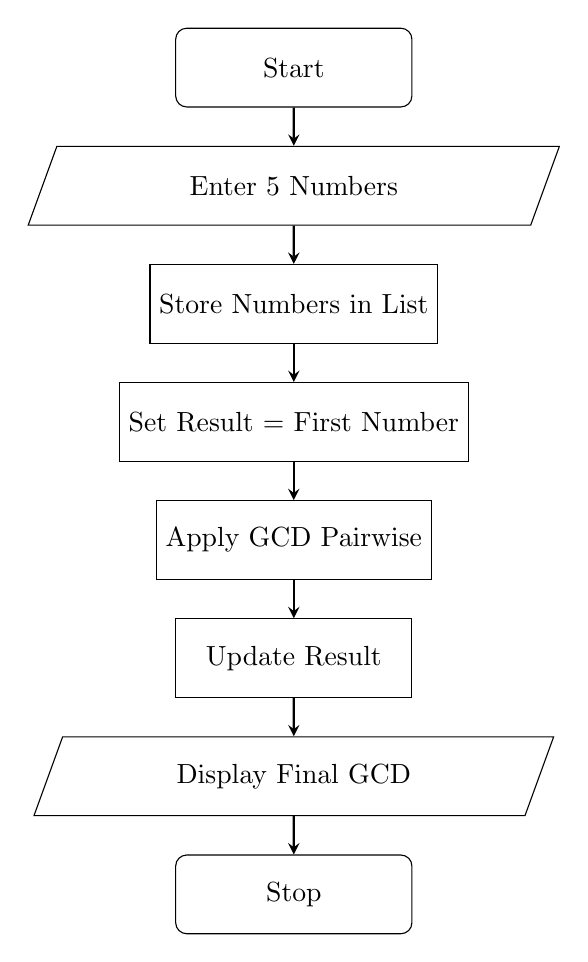
\begin{tikzpicture}[node distance=1.5cm]

\node (start) [startstop] {Start};

\node (input) [inputoutput, below of=start]
{Enter 5 Numbers};

\node (process1) [process, below of=input]
{Store Numbers in List};

\node (process2) [process, below of=process1]
{Set Result = First Number};

\node (process3) [process, below of=process2]
{Apply GCD Pairwise};

\node (process4) [process, below of=process3]
{Update Result};

\node (output) [inputoutput, below of=process4]
{Display Final GCD};

\node (stop) [startstop, below of=output]
{Stop};

\draw [arrow] (start) -- (input);
\draw [arrow] (input) -- (process1);
\draw [arrow] (process1) -- (process2);
\draw [arrow] (process2) -- (process3);
\draw [arrow] (process3) -- (process4);
\draw [arrow] (process4) -- (output);
\draw [arrow] (output) -- (stop);

\end{tikzpicture}
\end{center}
}

\newcommand{\flowtwentynine}{
\begin{center}
\begin{tikzpicture}[node distance=1.5cm]

\node (start) [startstop] {Start};

\node (init) [process, below of=start]
{Create FruitStore Object};

\node (input1) [inputoutput, below of=init]
{Enter Number of Fruits};

\node (loop) [process, below of=input1]
{Repeat for Each Fruit};

\node (input2) [inputoutput, below of=loop]
{Enter Name and Price};

\node (decision) [decision, below of=input2, yshift=-2.0cm]
{Fruit already exists?};

\node (add) [process, below of=decision, yshift= -2.0cm]
{Add Fruit to Dictionary};

\node (error) [inputoutput, right of=decision, xshift=7cm]
{Show Error Message};

\node (output) [inputoutput, below of=add, yshift= -1.0cm]
{Display Fruit List};

\node (stop) [startstop, below of=output]
{Stop};

\draw [arrow] (start) -- (init);
\draw [arrow] (init) -- (input1);
\draw [arrow] (input1) -- (loop);
\draw [arrow] (loop) -- (input2);
\draw [arrow] (input2) -- (decision);

\draw [arrow] (decision) -- node[left]{No} (add);
\draw [arrow] (decision) -- node[above]{Yes} (error);

\draw [arrow] (add) -- (output);
\draw [arrow] (error) |- (output);

\draw [arrow] (output) -- (stop);

\end{tikzpicture}
\end{center}
}

\newcommand{\flowthirty}{
\begin{center}
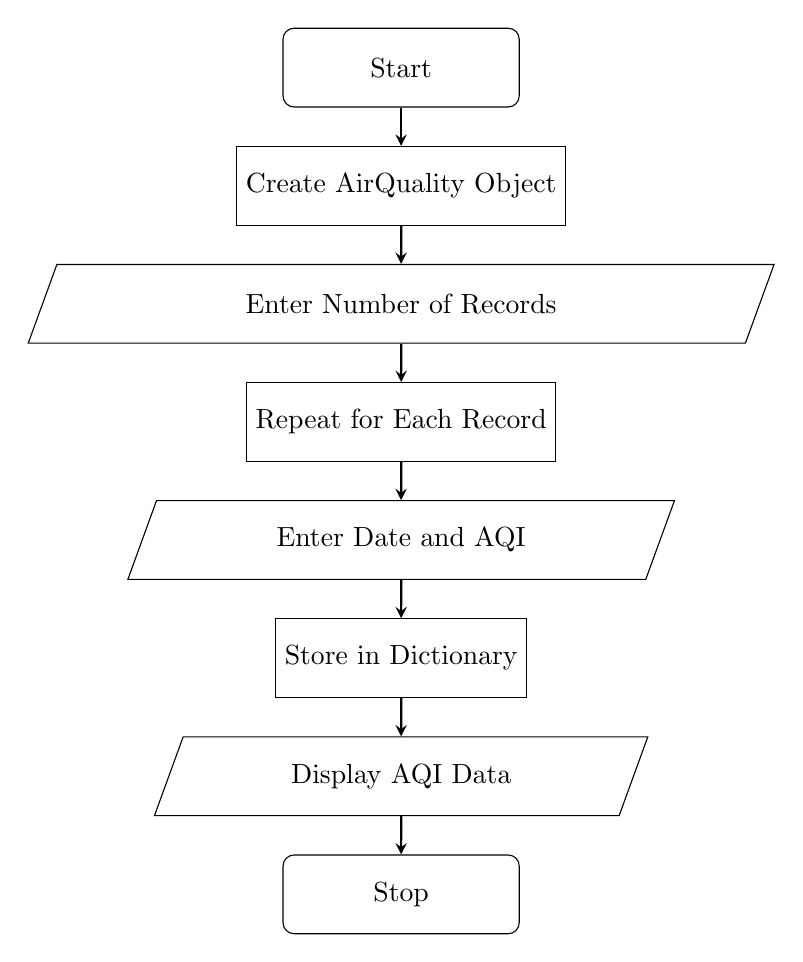
\begin{tikzpicture}[node distance=1.5cm]

\node (start) [startstop] {Start};

\node (init) [process, below of=start]
{Create AirQuality Object};

\node (input1) [inputoutput, below of=init]
{Enter Number of Records};

\node (loop) [process, below of=input1]
{Repeat for Each Record};

\node (input2) [inputoutput, below of=loop]
{Enter Date and AQI};

\node (process1) [process, below of=input2]
{Store in Dictionary};

\node (output) [inputoutput, below of=process1]
{Display AQI Data};

\node (stop) [startstop, below of=output]
{Stop};

\draw [arrow] (start) -- (init);
\draw [arrow] (init) -- (input1);
\draw [arrow] (input1) -- (loop);
\draw [arrow] (loop) -- (input2);
\draw [arrow] (input2) -- (process1);
\draw [arrow] (process1) -- (output);
\draw [arrow] (output) -- (stop);

\end{tikzpicture}
\end{center}
}

\newcommand{\flowthirtyone}{
\begin{center}
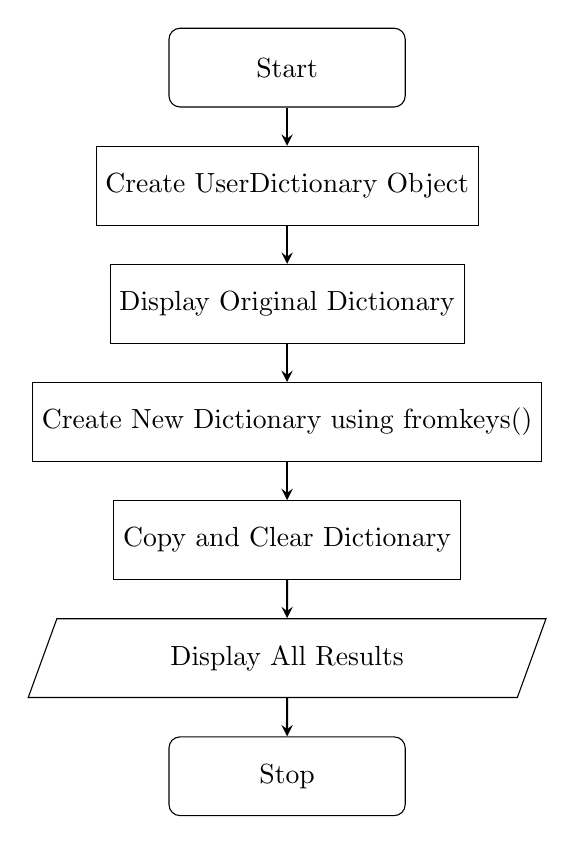
\begin{tikzpicture}[node distance=1.5cm]

\node (start) [startstop] {Start};

\node (init) [process, below of=start]
{Create UserDictionary Object};

\node (show) [process, below of=init]
{Display Original Dictionary};

\node (fromkeys) [process, below of=show]
{Create New Dictionary using fromkeys()};

\node (clear) [process, below of=fromkeys]
{Copy and Clear Dictionary};

\node (output) [inputoutput, below of=clear]
{Display All Results};

\node (stop) [startstop, below of=output]
{Stop};

\draw [arrow] (start) -- (init);
\draw [arrow] (init) -- (show);
\draw [arrow] (show) -- (fromkeys);
\draw [arrow] (fromkeys) -- (clear);
\draw [arrow] (clear) -- (output);
\draw [arrow] (output) -- (stop);

\end{tikzpicture}
\end{center}
}

\newcommand{\flowthirtytwo}{
\begin{center}
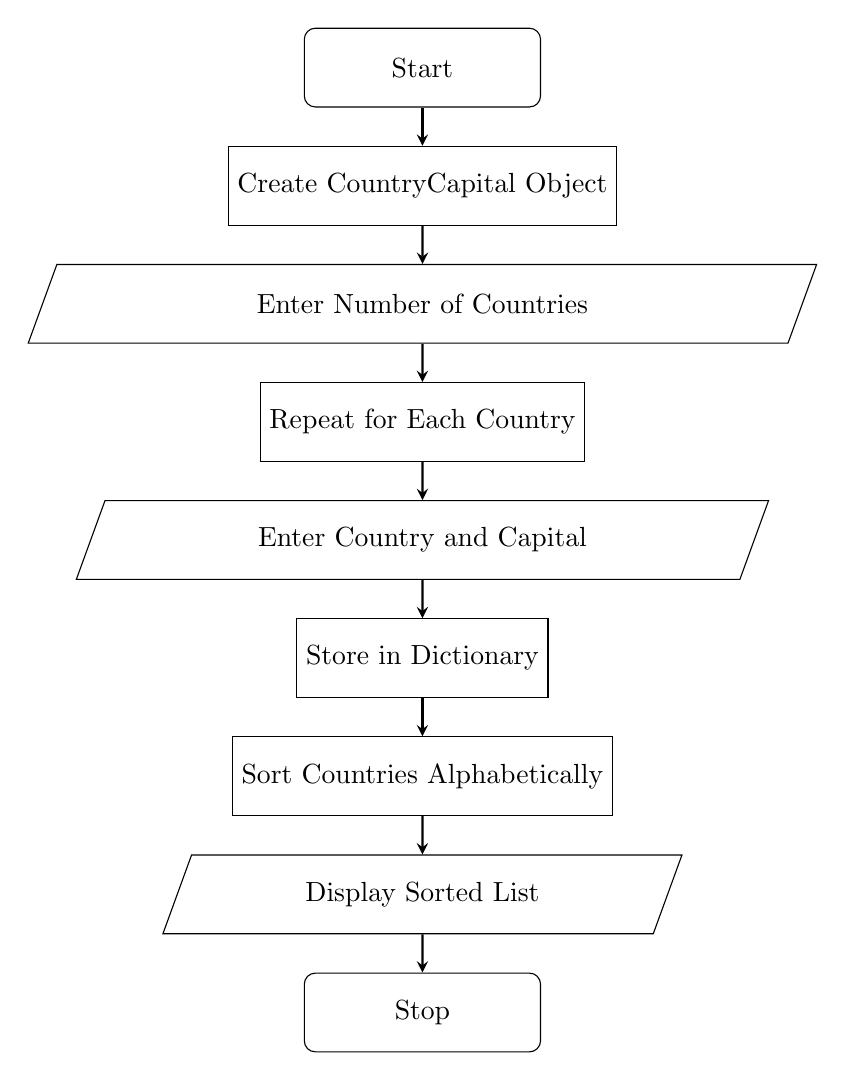
\begin{tikzpicture}[node distance=1.5cm]

\node (start) [startstop] {Start};

\node (init) [process, below of=start]
{Create CountryCapital Object};

\node (input1) [inputoutput, below of=init]
{Enter Number of Countries};

\node (loop) [process, below of=input1]
{Repeat for Each Country};

\node (input2) [inputoutput, below of=loop]
{Enter Country and Capital};

\node (store) [process, below of=input2]
{Store in Dictionary};

\node (sort) [process, below of=store]
{Sort Countries Alphabetically};

\node (output) [inputoutput, below of=sort]
{Display Sorted List};

\node (stop) [startstop, below of=output]
{Stop};

\draw [arrow] (start) -- (init);
\draw [arrow] (init) -- (input1);
\draw [arrow] (input1) -- (loop);
\draw [arrow] (loop) -- (input2);
\draw [arrow] (input2) -- (store);
\draw [arrow] (store) -- (sort);
\draw [arrow] (sort) -- (output);
\draw [arrow] (output) -- (stop);

\end{tikzpicture}
\end{center}
}

\newcommand{\flowthirtythree}{
\begin{center}
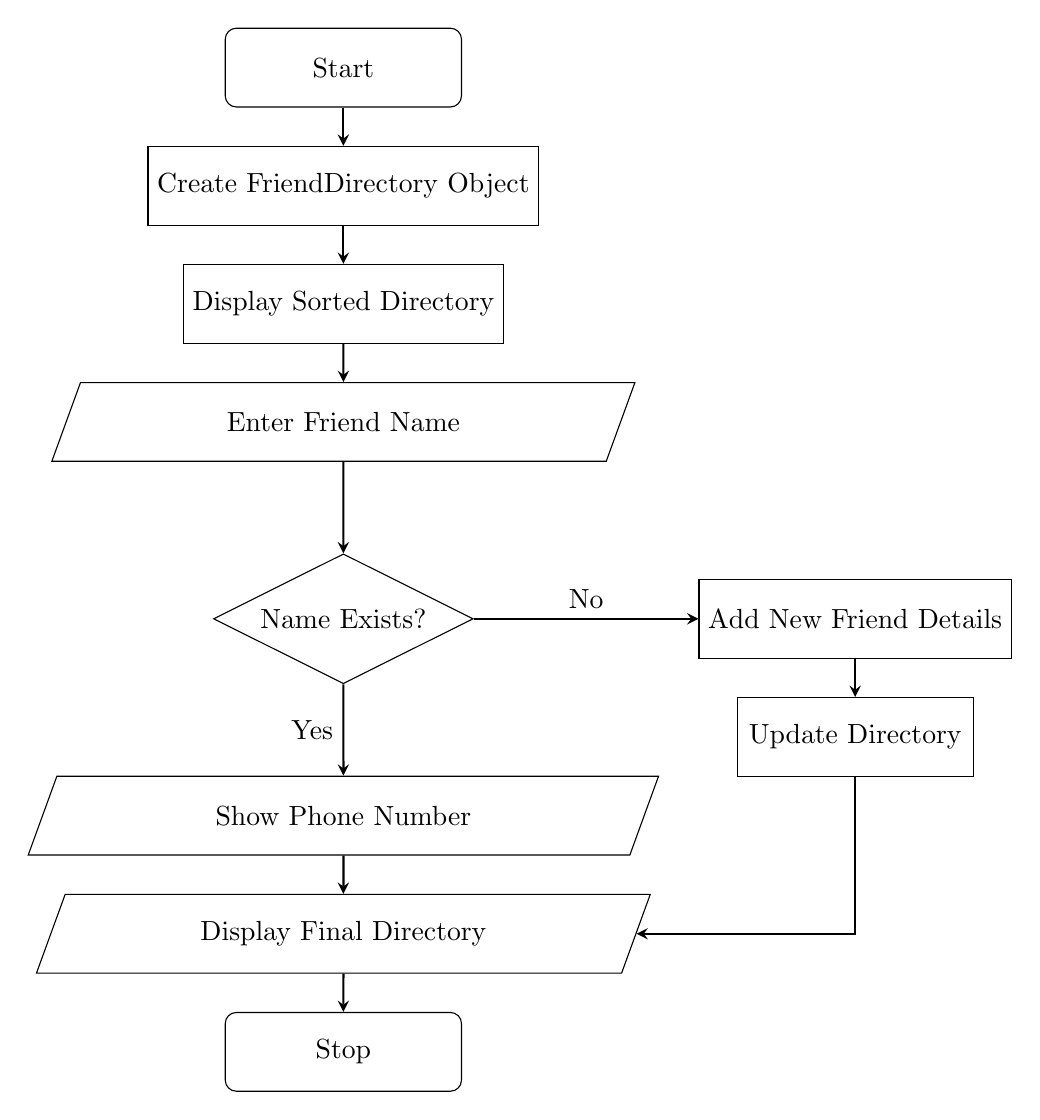
\begin{tikzpicture}[node distance=1.5cm]

\node (start) [startstop] {Start};

\node (init) [process, below of=start]
{Create FriendDirectory Object};

\node (display) [process, below of=init]
{Display Sorted Directory};

\node (input) [inputoutput, below of=display]
{Enter Friend Name};

\node (decision) [decision, below of=input, yshift=-1cm]
{Name Exists?};

\node (found) [inputoutput, below of=decision, yshift=-1cm]
{Show Phone Number};

\node (add) [process, right of=decision, xshift=5cm]
{Add New Friend Details};

\node (update) [process, below of=add]
{Update Directory};

\node (output) [inputoutput, below of=found]
{Display Final Directory};

\node (stop) [startstop, below of=output]
{Stop};

\draw [arrow] (start) -- (init);
\draw [arrow] (init) -- (display);
\draw [arrow] (display) -- (input);
\draw [arrow] (input) -- (decision);

\draw [arrow] (decision) -- node[left]{Yes} (found);
\draw [arrow] (decision) -- node[above]{No} (add);

\draw [arrow] (found) -- (output);
\draw [arrow] (add) -- (update);
\draw [arrow] (update) |- (output);

\draw [arrow] (output) -- (stop);

\end{tikzpicture}
\end{center}
}

\newcommand{\flowthirtyfour}{
\begin{center}
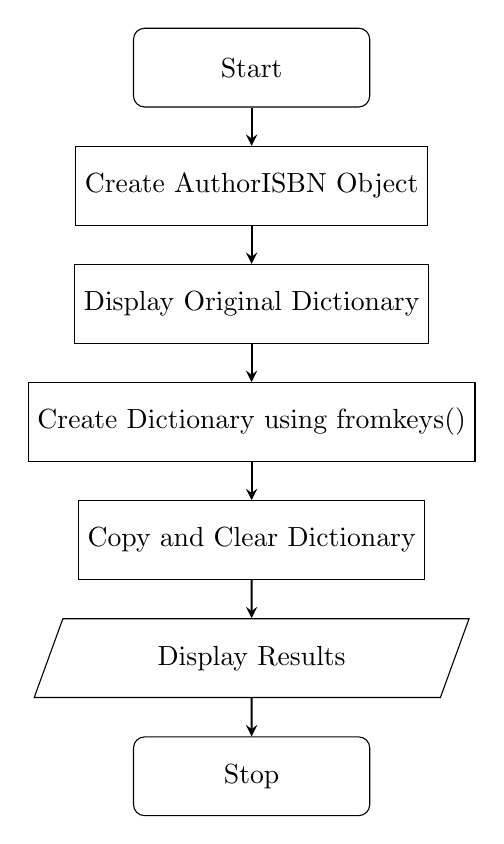
\begin{tikzpicture}[node distance=1.5cm]

\node (start) [startstop] {Start};

\node (init) [process, below of=start]
{Create AuthorISBN Object};

\node (show) [process, below of=init]
{Display Original Dictionary};

\node (fromkeys) [process, below of=show]
{Create Dictionary using fromkeys()};

\node (clear) [process, below of=fromkeys]
{Copy and Clear Dictionary};

\node (output) [inputoutput, below of=clear]
{Display Results};

\node (stop) [startstop, below of=output]
{Stop};

\draw [arrow] (start) -- (init);
\draw [arrow] (init) -- (show);
\draw [arrow] (show) -- (fromkeys);
\draw [arrow] (fromkeys) -- (clear);
\draw [arrow] (clear) -- (output);
\draw [arrow] (output) -- (stop);

\end{tikzpicture}
\end{center}
}

\newcommand{\flowthirtyfive}{
\begin{center}
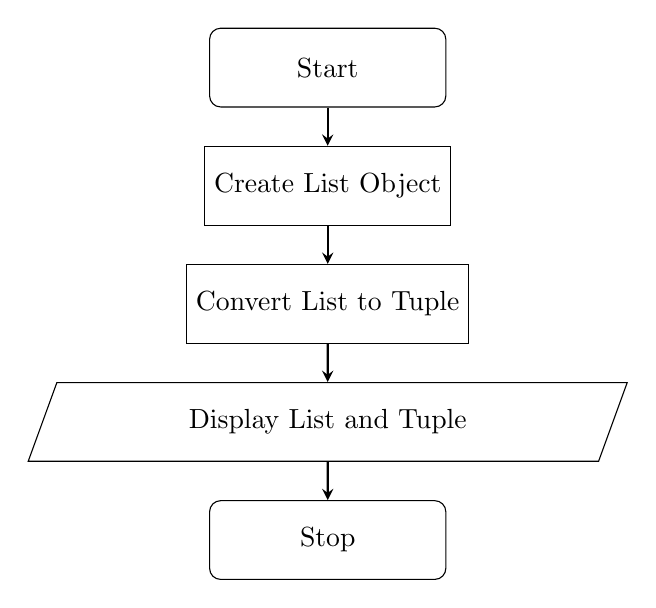
\begin{tikzpicture}[node distance=1.5cm]

\node (start) [startstop] {Start};

\node (process1) [process, below of=start]
{Create List Object};

\node (process2) [process, below of=process1]
{Convert List to Tuple};

\node (output) [inputoutput, below of=process2]
{Display List and Tuple};

\node (stop) [startstop, below of=output]
{Stop};

\draw [arrow] (start) -- (process1);
\draw [arrow] (process1) -- (process2);
\draw [arrow] (process2) -- (output);
\draw [arrow] (output) -- (stop);

\end{tikzpicture}
\end{center}
}

\newcommand{\flowthirtysix}{
\begin{center}
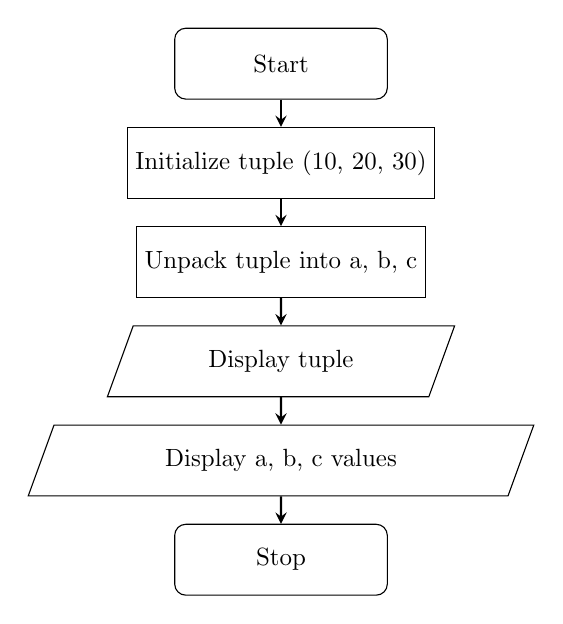
\begin{tikzpicture}[node distance=1.4cm, scale=0.9, transform shape]

\node (start) [startstop] {Start};

\node (init) [process, below of=start] 
{Initialize tuple (10, 20, 30)};

\node (unpack) [process, below of=init] 
{Unpack tuple into a, b, c};

\node (display1) [inputoutput, below of=unpack] 
{Display tuple};

\node (display2) [inputoutput, below of=display1] 
{Display a, b, c values};

\node (stop) [startstop, below of=display2] {Stop};

\draw [arrow] (start) -- (init);
\draw [arrow] (init) -- (unpack);
\draw [arrow] (unpack) -- (display1);
\draw [arrow] (display1) -- (display2);
\draw [arrow] (display2) -- (stop);

\end{tikzpicture}
\end{center}
}

\newcommand{\flowthirtyseven}{
\begin{center}
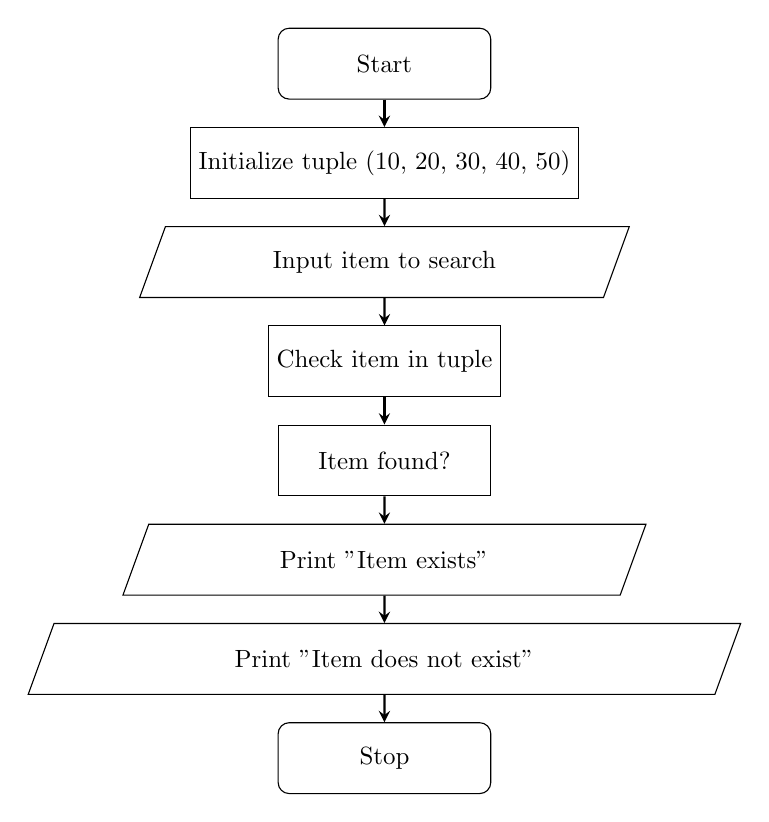
\begin{tikzpicture}[node distance=1.4cm, scale=0.9, transform shape]

\node (start) [startstop] {Start};

\node (init) [process, below of=start] 
{Initialize tuple (10, 20, 30, 40, 50)};

\node (input) [inputoutput, below of=init] 
{Input item to search};

\node (check) [process, below of=input] 
{Check item in tuple};

\node (decision) [process, below of=check] 
{Item found?};

\node (yes) [inputoutput, below of=decision] 
{Print "Item exists"};

\node (no) [inputoutput, below of=yes] 
{Print "Item does not exist"};

\node (stop) [startstop, below of=no] {Stop};

\draw [arrow] (start) -- (init);
\draw [arrow] (init) -- (input);
\draw [arrow] (input) -- (check);
\draw [arrow] (check) -- (decision);
\draw [arrow] (decision) -- (yes);
\draw [arrow] (yes) -- (no);
\draw [arrow] (no) -- (stop);

\end{tikzpicture}
\end{center}
}

\newcommand{\flowthirtyeight}{
\begin{center}
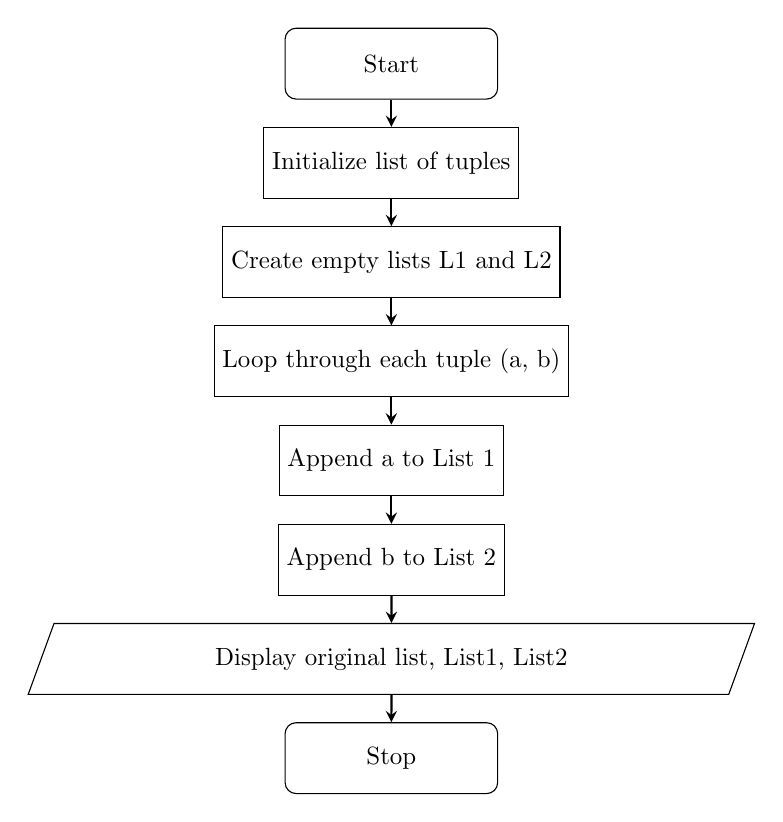
\begin{tikzpicture}[node distance=1.4cm, scale=0.9, transform shape]

\node (start) [startstop] {Start};

\node (init) [process, below of=start] 
{Initialize list of tuples};

\node (split) [process, below of=init] 
{Create empty lists L1 and L2};

\node (loop) [process, below of=split] 
{Loop through each tuple (a, b)};

\node (store1) [process, below of=loop] 
{Append a to List 1};

\node (store2) [process, below of=store1] 
{Append b to List 2};

\node (output) [inputoutput, below of=store2] 
{Display original list, List1, List2};

\node (stop) [startstop, below of=output] {Stop};

\draw [arrow] (start) -- (init);
\draw [arrow] (init) -- (split);
\draw [arrow] (split) -- (loop);
\draw [arrow] (loop) -- (store1);
\draw [arrow] (store1) -- (store2);
\draw [arrow] (store2) -- (output);
\draw [arrow] (output) -- (stop);

\end{tikzpicture}
\end{center}
}

\newcommand{\flowthirtynine}{
\begin{center}
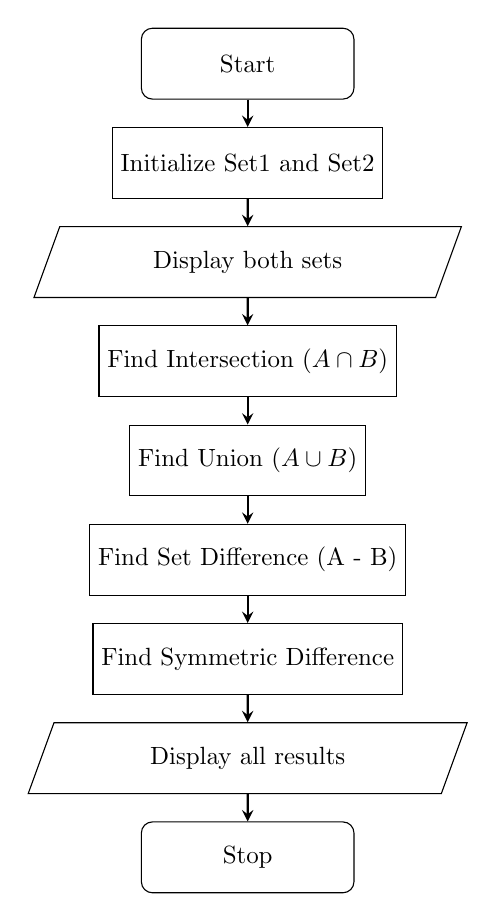
\begin{tikzpicture}[node distance=1.4cm, scale=0.9, transform shape]

\node (start) [startstop] {Start};

\node (init) [process, below of=start] 
{Initialize Set1 and Set2};

\node (display) [inputoutput, below of=init] 
{Display both sets};

\node (inter) [process, below of=display] 
{Find Intersection $(A \cap B)$};

\node (union) [process, below of=inter] 
{Find Union $(A \cup B)$};

\node (diff) [process, below of=union] 
{Find Set Difference (A - B)};

\node (sym) [process, below of=diff] 
{Find Symmetric Difference};

\node (output) [inputoutput, below of=sym] 
{Display all results};

\node (stop) [startstop, below of=output] {Stop};

\draw [arrow] (start) -- (init);
\draw [arrow] (init) -- (display);
\draw [arrow] (display) -- (inter);
\draw [arrow] (inter) -- (union);
\draw [arrow] (union) -- (diff);
\draw [arrow] (diff) -- (sym);
\draw [arrow] (sym) -- (output);
\draw [arrow] (output) -- (stop);

\end{tikzpicture}
\end{center}
}

\newcommand{\flowforty}{
\begin{center}
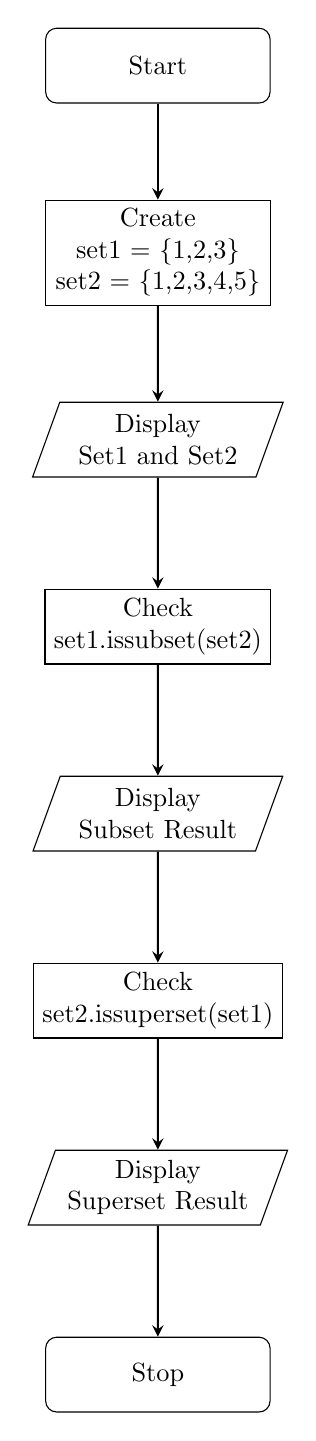
\begin{tikzpicture}[node distance=2.5cm, scale=0.95, transform shape]

\node (start) [startstop] {Start};

\node (create) [process, below of=start, align=center]
{Create\\
set1 = \{1,2,3\}\\
set2 = \{1,2,3,4,5\}};

\node (display) [inputoutput, below of=create, align=center]
{Display\\
Set1 and Set2};

\node (subset) [process, below of=display, align=center]
{Check\\
set1.issubset(set2)};

\node (subresult) [inputoutput, below of=subset, align=center]
{Display\\
Subset Result};

\node (superset) [process, below of=subresult, align=center]
{Check\\
set2.issuperset(set1)};

\node (superesult) [inputoutput, below of=superset, align=center]
{Display\\
Superset Result};

\node (stop) [startstop, below of=superesult]
{Stop};

% Arrows
\draw [arrow] (start) -- (create);
\draw [arrow] (create) -- (display);
\draw [arrow] (display) -- (subset);
\draw [arrow] (subset) -- (subresult);
\draw [arrow] (subresult) -- (superset);
\draw [arrow] (superset) -- (superesult);
\draw [arrow] (superesult) -- (stop);

\end{tikzpicture}
\end{center}
}

\newcommand{\flowfortyone}{
\begin{center}
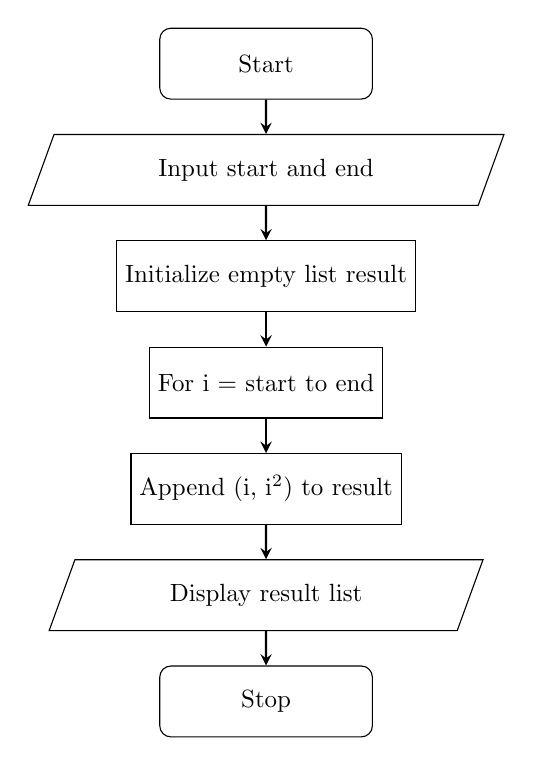
\begin{tikzpicture}[node distance=1.5cm, scale=0.9, transform shape]

\node (start) [startstop] {Start};

\node (input) [inputoutput, below of=start] 
{Input start and end};

\node (init) [process, below of=input] 
{Initialize empty list result};

\node (loop) [process, below of=init] 
{For i = start to end};

\node (process) [process, below of=loop] 
{Append (i, i$^2$) to result};

\node (output) [inputoutput, below of=process] 
{Display result list};

\node (stop) [startstop, below of=output] {Stop};

\draw [arrow] (start) -- (input);
\draw [arrow] (input) -- (init);
\draw [arrow] (init) -- (loop);
\draw [arrow] (loop) -- (process);
\draw [arrow] (process) -- (output);
\draw [arrow] (output) -- (stop);

\end{tikzpicture}
\end{center}
}

\newcommand{\flowfortytwo}{
\begin{center}
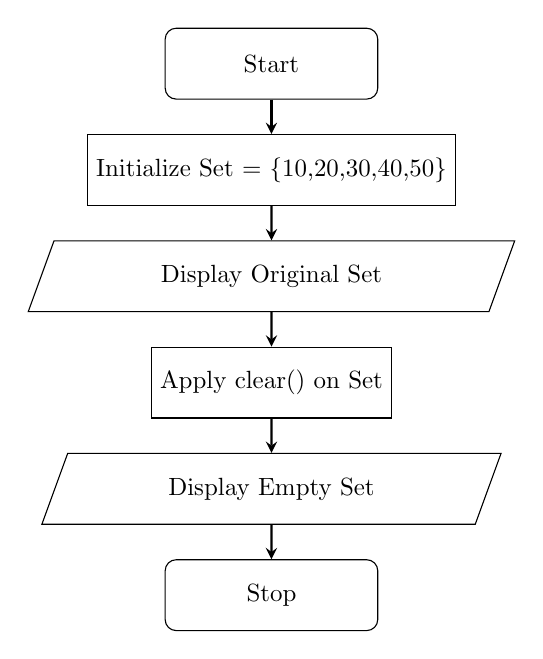
\begin{tikzpicture}[node distance=1.5cm, scale=0.9, transform shape]

\node (start) [startstop] {Start};

\node (init) [process, below of=start] 
{Initialize Set = \{10,20,30,40,50\}};

\node (print1) [inputoutput, below of=init] 
{Display Original Set};

\node (clear) [process, below of=print1] 
{Apply clear() on Set};

\node (print2) [inputoutput, below of=clear] 
{Display Empty Set};

\node (stop) [startstop, below of=print2] {Stop};

\draw [arrow] (start) -- (init);
\draw [arrow] (init) -- (print1);
\draw [arrow] (print1) -- (clear);
\draw [arrow] (clear) -- (print2);
\draw [arrow] (print2) -- (stop);

\end{tikzpicture}
\end{center}
}

\newcommand{\flowfortythree}{
\begin{center}
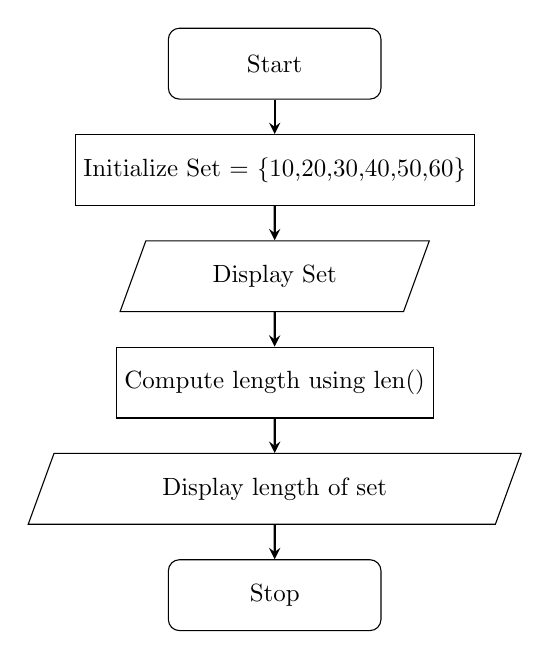
\begin{tikzpicture}[node distance=1.5cm, scale=0.9, transform shape]

\node (start) [startstop] {Start};

\node (init) [process, below of=start] 
{Initialize Set = \{10,20,30,40,50,60\}};

\node (print1) [inputoutput, below of=init] 
{Display Set};

\node (len) [process, below of=print1] 
{Compute length using len()};

\node (output) [inputoutput, below of=len] 
{Display length of set};

\node (stop) [startstop, below of=output] {Stop};

\draw [arrow] (start) -- (init);
\draw [arrow] (init) -- (print1);
\draw [arrow] (print1) -- (len);
\draw [arrow] (len) -- (output);
\draw [arrow] (output) -- (stop);

\end{tikzpicture}
\end{center}
}

\newcommand{\flowfortyfour}{
\begin{center}
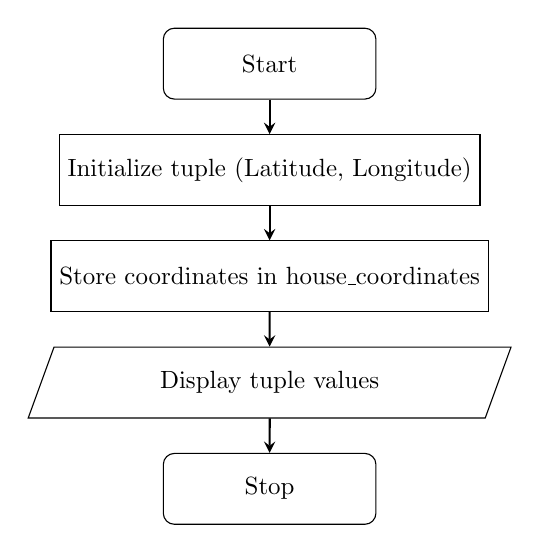
\begin{tikzpicture}[node distance=1.5cm, scale=0.9, transform shape]

\node (start) [startstop] {Start};

\node (init) [process, below of=start] 
{Initialize tuple (Latitude, Longitude)};

\node (store) [process, below of=init] 
{Store coordinates in house\_coordinates};

\node (display) [inputoutput, below of=store] 
{Display tuple values};

\node (stop) [startstop, below of=display] {Stop};

\draw [arrow] (start) -- (init);
\draw [arrow] (init) -- (store);
\draw [arrow] (store) -- (display);
\draw [arrow] (display) -- (stop);

\end{tikzpicture}
\end{center}
}

\newcommand{\flowfortyfive}{
\begin{center}
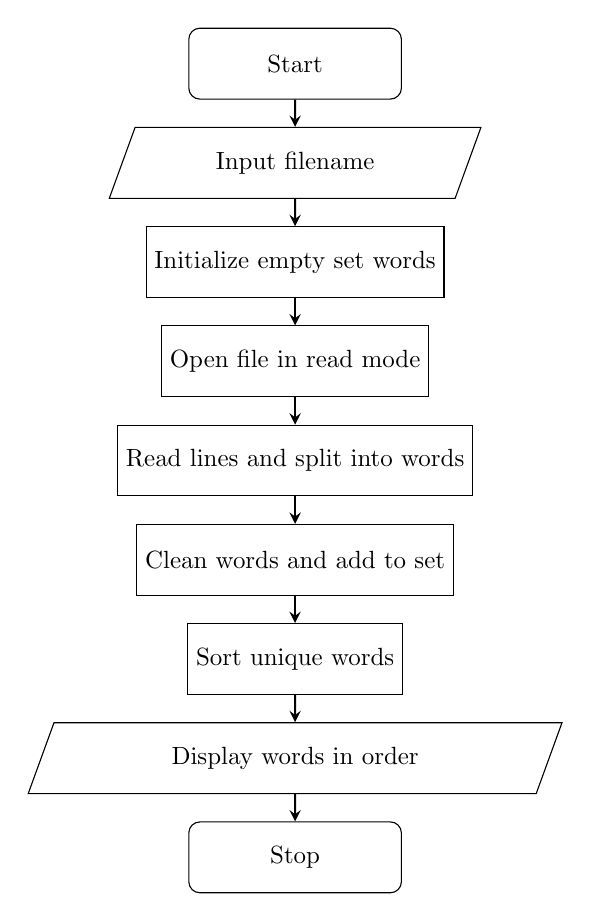
\begin{tikzpicture}[node distance=1.4cm, scale=0.9, transform shape]

\node (start) [startstop] {Start};

\node (input) [inputoutput, below of=start] 
{Input filename};

\node (init) [process, below of=input] 
{Initialize empty set words};

\node (open) [process, below of=init] 
{Open file in read mode};

\node (read) [process, below of=open] 
{Read lines and split into words};

\node (clean) [process, below of=read] 
{Clean words and add to set};

\node (sort) [process, below of=clean] 
{Sort unique words};

\node (output) [inputoutput, below of=sort] 
{Display words in order};

\node (stop) [startstop, below of=output] {Stop};

\draw [arrow] (start) -- (input);
\draw [arrow] (input) -- (init);
\draw [arrow] (init) -- (open);
\draw [arrow] (open) -- (read);
\draw [arrow] (read) -- (clean);
\draw [arrow] (clean) -- (sort);
\draw [arrow] (sort) -- (output);
\draw [arrow] (output) -- (stop);

\end{tikzpicture}
\end{center}
}

\newcommand{\flowfortysix}{
\begin{center}
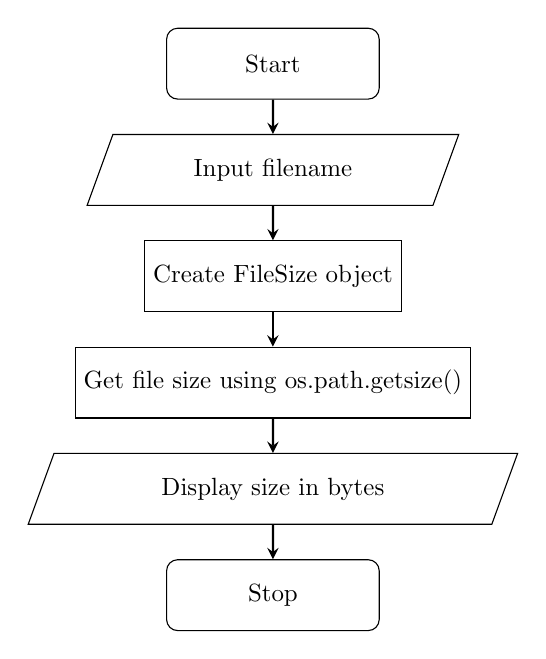
\begin{tikzpicture}[node distance=1.5cm, scale=0.9, transform shape]

\node (start) [startstop] {Start};

\node (input) [inputoutput, below of=start] 
{Input filename};

\node (init) [process, below of=input] 
{Create FileSize object};

\node (size) [process, below of=init] 
{Get file size using os.path.getsize()};

\node (output) [inputoutput, below of=size] 
{Display size in bytes};

\node (stop) [startstop, below of=output] {Stop};

\draw [arrow] (start) -- (input);
\draw [arrow] (input) -- (init);
\draw [arrow] (init) -- (size);
\draw [arrow] (size) -- (output);
\draw [arrow] (output) -- (stop);

\end{tikzpicture}
\end{center}
}

\newcommand{\flowfortyseven}{
\begin{center}
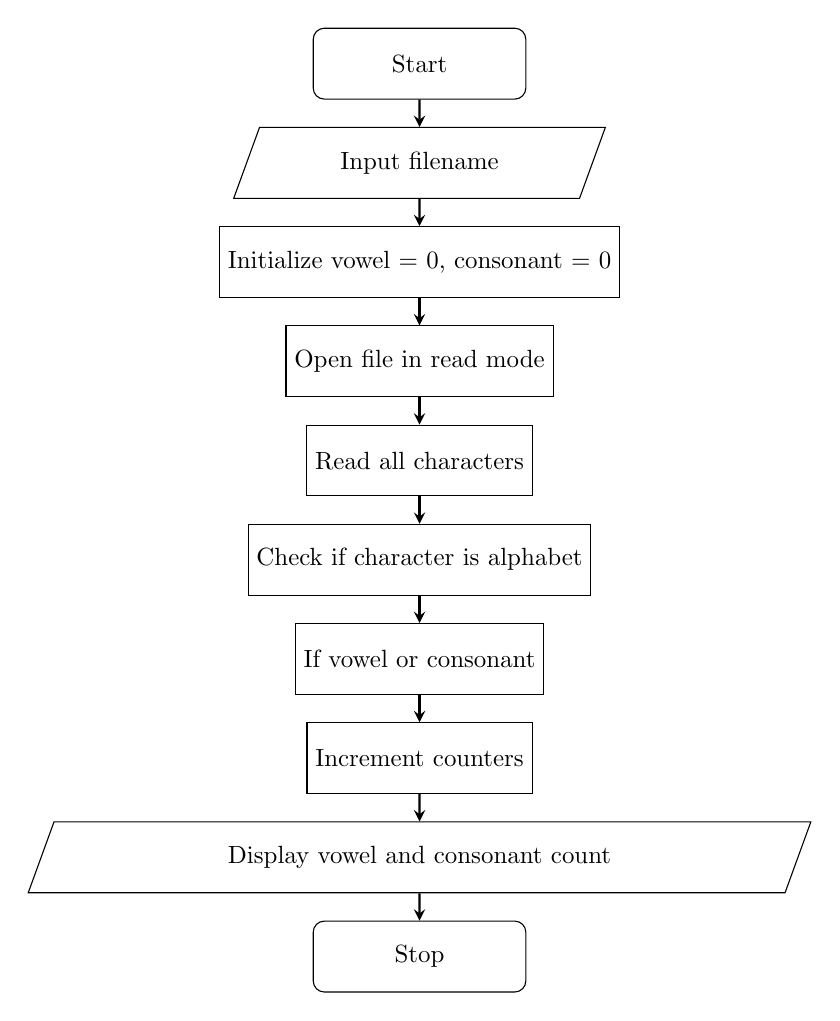
\begin{tikzpicture}[node distance=1.4cm, scale=0.9, transform shape]

\node (start) [startstop] {Start};

\node (input) [inputoutput, below of=start] 
{Input filename};

\node (init) [process, below of=input] 
{Initialize vowel = 0, consonant = 0};

\node (open) [process, below of=init] 
{Open file in read mode};

\node (read) [process, below of=open] 
{Read all characters};

\node (check) [process, below of=read] 
{Check if character is alphabet};

\node (decision) [process, below of=check] 
{If vowel or consonant};

\node (count) [process, below of=decision] 
{Increment counters};

\node (output) [inputoutput, below of=count] 
{Display vowel and consonant count};

\node (stop) [startstop, below of=output] {Stop};

\draw [arrow] (start) -- (input);
\draw [arrow] (input) -- (init);
\draw [arrow] (init) -- (open);
\draw [arrow] (open) -- (read);
\draw [arrow] (read) -- (check);
\draw [arrow] (check) -- (decision);
\draw [arrow] (decision) -- (count);
\draw [arrow] (count) -- (output);
\draw [arrow] (output) -- (stop);

\end{tikzpicture}
\end{center}
}
\newcommand{\flowfortyeight}{
\begin{center}
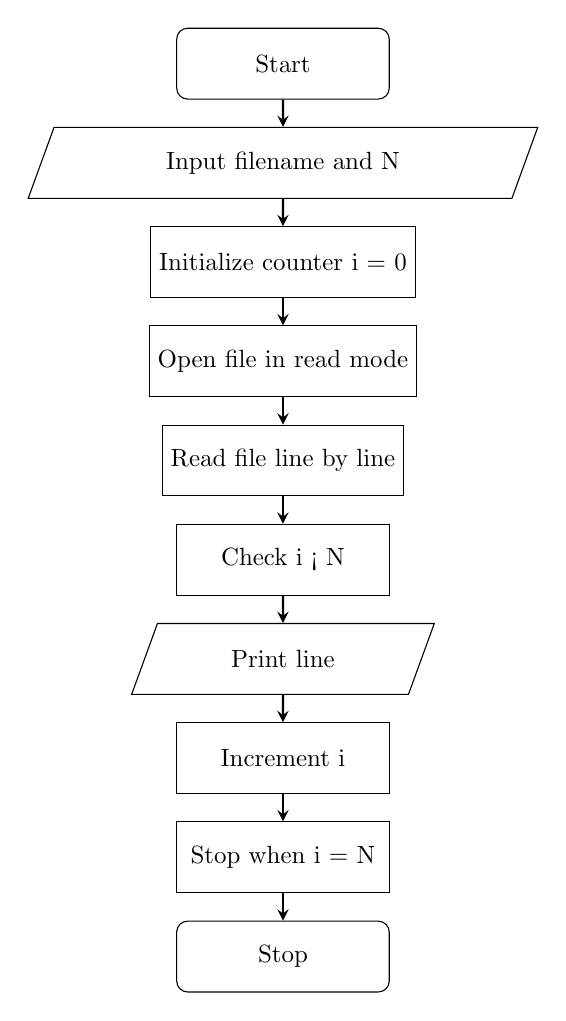
\begin{tikzpicture}[node distance=1.4cm, scale=0.9, transform shape]

\node (start) [startstop] {Start};

\node (input) [inputoutput, below of=start] 
{Input filename and N};

\node (init) [process, below of=input] 
{Initialize counter i = 0};

\node (open) [process, below of=init] 
{Open file in read mode};

\node (read) [process, below of=open] 
{Read file line by line};

\node (check) [process, below of=read] 
{Check i < N};

\node (print) [inputoutput, below of=check] 
{Print line};

\node (inc) [process, below of=print] 
{Increment i};

\node (stopcond) [process, below of=inc] 
{Stop when i = N};

\node (stop) [startstop, below of=stopcond] {Stop};

\draw [arrow] (start) -- (input);
\draw [arrow] (input) -- (init);
\draw [arrow] (init) -- (open);
\draw [arrow] (open) -- (read);
\draw [arrow] (read) -- (check);
\draw [arrow] (check) -- (print);
\draw [arrow] (print) -- (inc);
\draw [arrow] (inc) -- (stopcond);
\draw [arrow] (stopcond) -- (stop);

\end{tikzpicture}
\end{center}
}
\newcommand{\flowfortynine}{
\begin{center}
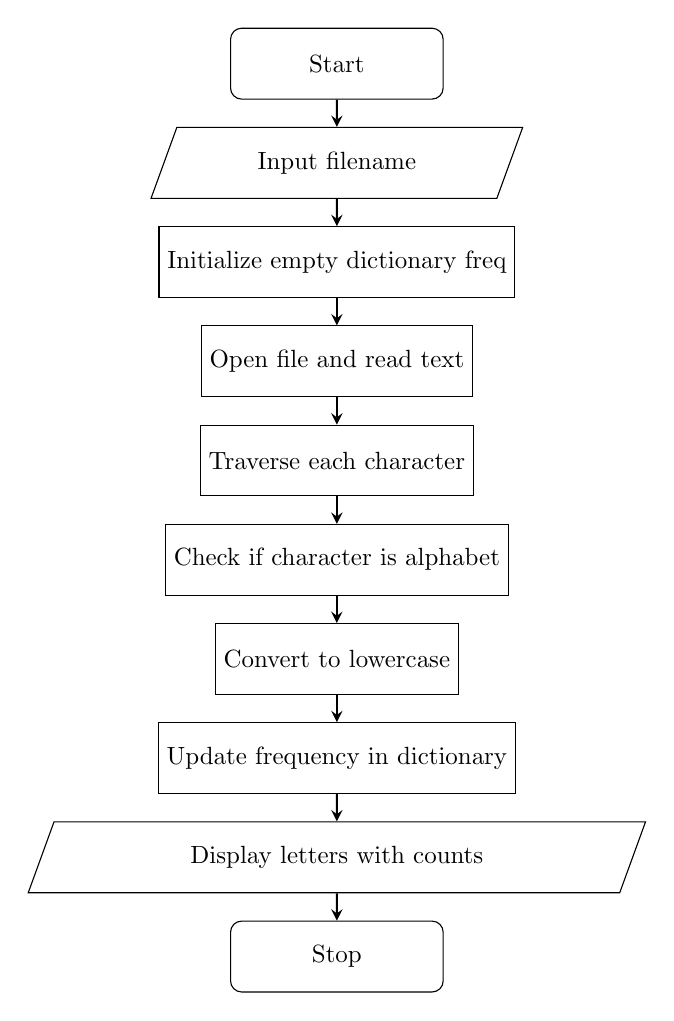
\begin{tikzpicture}[node distance=1.4cm, scale=0.9, transform shape]

\node (start) [startstop] {Start};

\node (input) [inputoutput, below of=start] 
{Input filename};

\node (init) [process, below of=input] 
{Initialize empty dictionary freq};

\node (open) [process, below of=init] 
{Open file and read text};

\node (loop) [process, below of=open] 
{Traverse each character};

\node (check) [process, below of=loop] 
{Check if character is alphabet};

\node (lower) [process, below of=check] 
{Convert to lowercase};

\node (update) [process, below of=lower] 
{Update frequency in dictionary};

\node (output) [inputoutput, below of=update] 
{Display letters with counts};

\node (stop) [startstop, below of=output] {Stop};

\draw [arrow] (start) -- (input);
\draw [arrow] (input) -- (init);
\draw [arrow] (init) -- (open);
\draw [arrow] (open) -- (loop);
\draw [arrow] (loop) -- (check);
\draw [arrow] (check) -- (lower);
\draw [arrow] (lower) -- (update);
\draw [arrow] (update) -- (output);
\draw [arrow] (output) -- (stop);

\end{tikzpicture}
\end{center}
}
\newcommand{\flowfifty}{
\begin{center}
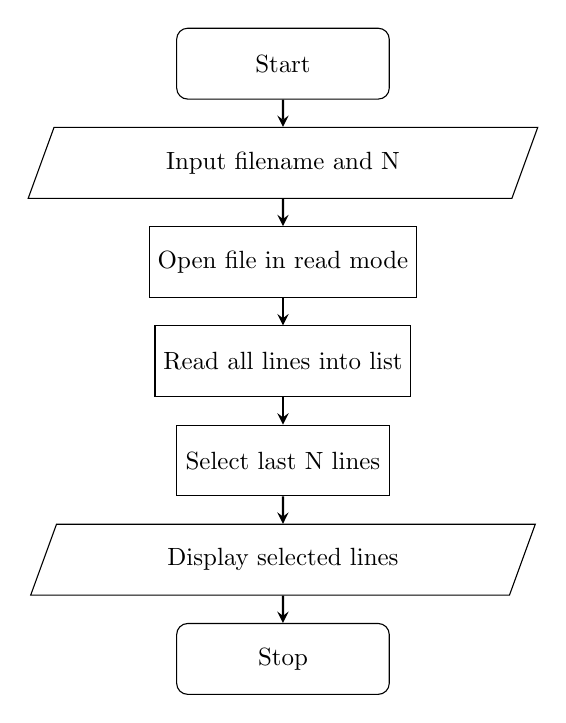
\begin{tikzpicture}[node distance=1.4cm, scale=0.9, transform shape]

\node (start) [startstop] {Start};

\node (input) [inputoutput, below of=start] 
{Input filename and N};

\node (open) [process, below of=input] 
{Open file in read mode};

\node (read) [process, below of=open] 
{Read all lines into list};

\node (slice) [process, below of=read] 
{Select last N lines};

\node (output) [inputoutput, below of=slice] 
{Display selected lines};

\node (stop) [startstop, below of=output] {Stop};

\draw [arrow] (start) -- (input);
\draw [arrow] (input) -- (open);
\draw [arrow] (open) -- (read);
\draw [arrow] (read) -- (slice);
\draw [arrow] (slice) -- (output);
\draw [arrow] (output) -- (stop);

\end{tikzpicture}
\end{center}
}
\newcommand{\flowfiftyone}{
\begin{center}
\begin{tikzpicture}[node distance=1.4cm, scale=0.9, transform shape]

\node (start) [startstop] {Start};

\node (input) [inputoutput, below of=start] 
{Input file1 and file2};

\node (open1) [process, below of=input] 
{Open file1 and read lines};

\node (open2) [process, below of=open1] 
{Open file2 and read lines};

\node (len) [process, below of=open2] 
{Find min length of both files};

\node (loop) [process, below of=len] 
{Loop from 0 to min length};

\node (print) [inputoutput, below of=loop] 
{Print paired lines};

\node (stop) [startstop, below of=print] {Stop};

\draw [arrow] (start) -- (input);
\draw [arrow] (input) -- (open1);
\draw [arrow] (open1) -- (open2);
\draw [arrow] (open2) -- (len);
\draw [arrow] (len) -- (loop);
\draw [arrow] (loop) -- (print);
\draw [arrow] (print) -- (stop);

\end{tikzpicture}
\end{center}
}

\newcommand{\flowfiftytwo}{
\begin{center}
\begin{tikzpicture}[node distance=2cm, scale=0.95, transform shape]

\node (start) [startstop] {Start};

\node (input) [inputoutput, below of=start]
{Input Filename};

\node (readfile) [process, below of=input, align=center]
{Open File\\
in Read Mode};

\node (readcontent) [process, below of=readfile]
{Read Content};

\node (replace) [process, below of=readcontent, align=center]
{Replace\\
\textbackslash n with Space};

\node (writefile) [process, below of=replace, align=center]
{Open File\\
in Write Mode};

\node (writecontent) [process, below of=writefile]
{Write Modified Content};

\node (message) [inputoutput, below of=writecontent, align=center]
{Display\\
"Newline Characters Removed"};

\node (stop) [startstop, below of=message]
{Stop};

% Arrows
\draw [arrow] (start) -- (input);
\draw [arrow] (input) -- (readfile);
\draw [arrow] (readfile) -- (readcontent);
\draw [arrow] (readcontent) -- (replace);
\draw [arrow] (replace) -- (writefile);
\draw [arrow] (writefile) -- (writecontent);
\draw [arrow] (writecontent) -- (message);
\draw [arrow] (message) -- (stop);

\end{tikzpicture}
\end{center}
}

\newcommand{\flowfiftythree}{
\begin{center}
\begin{tikzpicture}[node distance=1.4cm, scale=0.9, transform shape]

\node (start) [startstop] {Start};

\node (input) [inputoutput, below of=start] 
{Input filename};

\node (open) [process, below of=input] 
{Open file in read mode};

\node (read) [process, below of=open] 
{Read all lines into list};

\node (check) [process, below of=read] 
{Check if file is empty};

\node (random) [process, below of=check] 
{Select random line using random.choice()};

\node (output) [inputoutput, below of=random] 
{Display random line};

\node (stop) [startstop, below of=output] {Stop};

\draw [arrow] (start) -- (input);
\draw [arrow] (input) -- (open);
\draw [arrow] (open) -- (read);
\draw [arrow] (read) -- (check);
\draw [arrow] (check) -- (random);
\draw [arrow] (random) -- (output);
\draw [arrow] (output) -- (stop);

\end{tikzpicture}
\end{center}
}
\newcommand{\flowfiftyfour}{
\begin{center}
\begin{tikzpicture}[node distance=1.4cm, scale=0.9, transform shape]

\node (start) [startstop] {Start};

\node (input) [inputoutput, below of=start] 
{Input source and destination CSV files};

\node (open1) [process, below of=input] 
{Open source file in read mode};

\node (read) [process, below of=open1] 
{Read CSV data using csv.reader};

\node (open2) [process, below of=read] 
{Open destination file in write mode};

\node (write) [process, below of=open2] 
{Write data using csv.writer};

\node (output) [inputoutput, below of=write] 
{Display success message};

\node (stop) [startstop, below of=output] {Stop};

\draw [arrow] (start) -- (input);
\draw [arrow] (input) -- (open1);
\draw [arrow] (open1) -- (read);
\draw [arrow] (read) -- (open2);
\draw [arrow] (open2) -- (write);
\draw [arrow] (write) -- (output);
\draw [arrow] (output) -- (stop);

\end{tikzpicture}
\end{center}
}
\newcommand{\flowfiftyfive}{
\begin{center}
\begin{tikzpicture}[node distance=1.4cm, scale=0.9, transform shape]

\node (start) [startstop] {Start};

\node (input) [inputoutput, below of=start] 
{Input text};

\node (split) [process, below of=input] 
{Split text into words};

\node (init) [process, below of=split] 
{Compile regex pattern 'z'};

\node (loop) [process, below of=init] 
{Check each word};

\node (check) [process, below of=loop] 
{If word contains 'z' or 'Z'};

\node (store) [process, below of=check] 
{Add word to result list};

\node (output) [inputoutput, below of=store] 
{Display matching words};

\node (stop) [startstop, below of=output] {Stop};

\draw [arrow] (start) -- (input);
\draw [arrow] (input) -- (split);
\draw [arrow] (split) -- (init);
\draw [arrow] (init) -- (loop);
\draw [arrow] (loop) -- (check);
\draw [arrow] (check) -- (store);
\draw [arrow] (store) -- (output);
\draw [arrow] (output) -- (stop);

\end{tikzpicture}
\end{center}
}
\newcommand{\flowfiftysix}{
\begin{center}
\begin{tikzpicture}[node distance=1.4cm, scale=0.9, transform shape]

\node (start) [startstop] {Start};

\node (input) [inputoutput, below of=start] 
{Input IP address};

\node (split) [process, below of=input] 
{Split IP by "."};

\node (init) [process, below of=split] 
{Convert each part to int};

\node (clean) [process, below of=init] 
{Remove leading zeros};

\node (join) [process, below of=clean] 
{Join parts with "."};

\node (output) [inputoutput, below of=join] 
{Display updated IP};

\node (stop) [startstop, below of=output] {Stop};

\draw [arrow] (start) -- (input);
\draw [arrow] (input) -- (split);
\draw [arrow] (split) -- (init);
\draw [arrow] (init) -- (clean);
\draw [arrow] (clean) -- (join);
\draw [arrow] (join) -- (output);
\draw [arrow] (output) -- (stop);

\end{tikzpicture}
\end{center}
}
\newcommand{\flowfiftyseven}{
\begin{center}
\begin{tikzpicture}[node distance=1.4cm, scale=0.9, transform shape]

\node (start) [startstop] {Start};

\node (input) [inputoutput, below of=start] 
{Input text string};

\node (init) [process, below of=input] 
{Compile regex for 1–3 digit numbers};

\node (search) [process, below of=init] 
{Search numbers using findall()};

\node (store) [process, below of=search] 
{Store matched numbers in list};

\node (output) [inputoutput, below of=store] 
{Display extracted numbers};

\node (stop) [startstop, below of=output] {Stop};

\draw [arrow] (start) -- (input);
\draw [arrow] (input) -- (init);
\draw [arrow] (init) -- (search);
\draw [arrow] (search) -- (store);
\draw [arrow] (store) -- (output);
\draw [arrow] (output) -- (stop);

\end{tikzpicture}
\end{center}
}
\newcommand{\flowfiftyeight}{
\begin{center}
\begin{tikzpicture}[node distance=1.4cm, scale=0.9, transform shape]

\node (start) [startstop] {Start};

\node (input) [inputoutput, below of=start] 
{Input string};

\node (init) [process, below of=input] 
{Initialize empty list substrings};

\node (len) [process, below of=init] 
{Get length n of string};

\node (outer) [process, below of=len] 
{Loop i from 0 to n};

\node (inner) [process, below of=outer] 
{Loop j from i+1 to n};

\node (store) [process, below of=inner] 
{Append substring s[i:j]};

\node (output) [inputoutput, below of=store] 
{Display all substrings};

\node (stop) [startstop, below of=output] {Stop};

\draw [arrow] (start) -- (input);
\draw [arrow] (input) -- (init);
\draw [arrow] (init) -- (len);
\draw [arrow] (len) -- (outer);
\draw [arrow] (outer) -- (inner);
\draw [arrow] (inner) -- (store);
\draw [arrow] (store) -- (output);
\draw [arrow] (output) -- (stop);

\end{tikzpicture}
\end{center}
}
\newcommand{\flowfiftynine}{
\begin{center}
\begin{tikzpicture}[node distance=1.4cm, scale=0.9, transform shape]

\node (start) [startstop] {Start};

\node (input) [inputoutput, below of=start] 
{Input URL};

\node (init) [process, below of=input] 
{Define regex pattern YYYY-MM-DD};

\node (search) [process, below of=init] 
{Search date in URL using re.search()};

\node (check) [process, below of=search] 
{Check if match found};

\node (extract) [process, below of=check] 
{Extract Year, Month, Day};

\node (output1) [inputoutput, below of=extract] 
{Display Year, Month, Date};

\node (output2) [inputoutput, below of=output1] 
{Else: Display "No date found"};

\node (stop) [startstop, below of=output2] {Stop};

\draw [arrow] (start) -- (input);
\draw [arrow] (input) -- (init);
\draw [arrow] (init) -- (search);
\draw [arrow] (search) -- (check);
\draw [arrow] (check) -- (extract);
\draw [arrow] (extract) -- (output1);
\draw [arrow] (output1) -- (output2);
\draw [arrow] (output2) -- (stop);

\end{tikzpicture}
\end{center}
}
\newcommand{\flowsixty}{
\begin{center}
\begin{tikzpicture}[node distance=1.4cm, scale=0.9, transform shape]

\node (start) [startstop] {Start};

\node (input) [inputoutput, below of=start] 
{Input filename};

\node (openr) [process, below of=input] 
{Open file in read mode};

\node (read) [process, below of=openr] 
{Read entire file content};

\node (pattern) [process, below of=read] 
{Define regex YYYY-MM-DD};

\node (replace) [process, below of=pattern] 
{Replace date with DD-MM-YYYY};

\node (openw) [process, below of=replace] 
{Open file in write mode};

\node (write) [process, below of=openw] 
{Write updated content};

\node (output) [inputoutput, below of=write] 
{Display success message};

\node (stop) [startstop, below of=output] {Stop};

\draw [arrow] (start) -- (input);
\draw [arrow] (input) -- (openr);
\draw [arrow] (openr) -- (read);
\draw [arrow] (read) -- (pattern);
\draw [arrow] (pattern) -- (replace);
\draw [arrow] (replace) -- (openw);
\draw [arrow] (openw) -- (write);
\draw [arrow] (write) -- (output);
\draw [arrow] (output) -- (stop);

\end{tikzpicture}
\end{center}
}
\newcommand{\flowsixtyone}{
\begin{center}
\begin{tikzpicture}[node distance=1.4cm, scale=0.9, transform shape]

\node (start) [startstop] {Start};

\node (input) [inputoutput, below of=start] 
{Input text};

\node (pattern) [process, below of=input] 
{Define pattern: "Street"};

\node (replace) [process, below of=pattern] 
{Replace "Street" with "St." using re.sub()};

\node (output) [inputoutput, below of=replace] 
{Display updated text};

\node (stop) [startstop, below of=output] {Stop};

\draw [arrow] (start) -- (input);
\draw [arrow] (input) -- (pattern);
\draw [arrow] (pattern) -- (replace);
\draw [arrow] (replace) -- (output);
\draw [arrow] (output) -- (stop);

\end{tikzpicture}
\end{center}
}
\newcommand{\flowsixtytwo}{
\begin{center}
\begin{tikzpicture}[node distance=1.4cm, scale=0.9, transform shape]

\node (start) [startstop] {Start};

\node (input) [inputoutput, below of=start] 
{Input text};

\node (pattern) [process, below of=input] 
{Define regex: \textbackslash b\textbackslash w\{5\}\textbackslash b};

\node (search) [process, below of=pattern] 
{Find all matching words using re.findall()};

\node (store) [process, below of=search] 
{Store matched words in list};

\node (output) [inputoutput, below of=store] 
{Display five-letter words};

\node (stop) [startstop, below of=output] {Stop};

\draw [arrow] (start) -- (input);
\draw [arrow] (input) -- (pattern);
\draw [arrow] (pattern) -- (search);
\draw [arrow] (search) -- (store);
\draw [arrow] (store) -- (output);
\draw [arrow] (output) -- (stop);

\end{tikzpicture}
\end{center}
}
\newcommand{\flowsixtythree}{
\begin{center}
\begin{tikzpicture}[node distance=1.4cm, scale=0.9, transform shape]

\node (start) [startstop] {Start};

\node (input) [inputoutput, below of=start] 
{Input a, b, c};

\node (disc) [process, below of=input] 
{Compute discriminant $d = b^2 - 4ac$};

\node (sqrt) [process, below of=disc] 
{Compute $\sqrt{d}$ using cmath};

\node (root1) [process, below of=sqrt] 
{Compute Root 1};

\node (root2) [process, below of=root1] 
{Compute Root 2};

\node (output) [inputoutput, below of=root2] 
{Display both roots};

\node (stop) [startstop, below of=output] {Stop};

\draw [arrow] (start) -- (input);
\draw [arrow] (input) -- (disc);
\draw [arrow] (disc) -- (sqrt);
\draw [arrow] (sqrt) -- (root1);
\draw [arrow] (root1) -- (root2);
\draw [arrow] (root2) -- (output);
\draw [arrow] (output) -- (stop);

\end{tikzpicture}
\end{center}
}
\newcommand{\flowsixtyfour}{
\begin{center}
\begin{tikzpicture}[node distance=1.4cm, scale=0.9, transform shape]

\node (start) [startstop] {Start};

\node (inputn) [inputoutput, below of=start] 
{Input number of students n};

\node (loop) [process, below of=inputn] 
{Input name and marks (loop n times)};

\node (store) [process, below of=loop] 
{Store data in Student objects list};

\node (sort) [process, below of=store] 
{Sort students by marks (descending)};

\node (top5) [process, below of=sort] 
{Select top 5 students};

\node (output) [inputoutput, below of=top5] 
{Display name and marks};

\node (stop) [startstop, below of=output] {Stop};

\draw [arrow] (start) -- (inputn);
\draw [arrow] (inputn) -- (loop);
\draw [arrow] (loop) -- (store);
\draw [arrow] (store) -- (sort);
\draw [arrow] (sort) -- (top5);
\draw [arrow] (top5) -- (output);
\draw [arrow] (output) -- (stop);

\end{tikzpicture}
\end{center}
}
\newcommand{\flowsixtyfive}{
\begin{center}
\begin{tikzpicture}[node distance=1.4cm, scale=0.9, transform shape]

\node (start) [startstop] {Start};

\node (init) [process, below of=start] 
{Initialize Library object};

\node (input1) [inputoutput, below of=init] 
{Input acc no, title, author, publisher};

\node (input2) [inputoutput, below of=input1] 
{Input days late};

\node (calc) [process, below of=input2] 
{Compute fine = days $\times$ 1.50};

\node (output) [inputoutput, below of=calc] 
{Display fine amount};

\node (stop) [startstop, below of=output] {Stop};

\draw [arrow] (start) -- (init);
\draw [arrow] (init) -- (input1);
\draw [arrow] (input1) -- (input2);
\draw [arrow] (input2) -- (calc);
\draw [arrow] (calc) -- (output);
\draw [arrow] (output) -- (stop);

\end{tikzpicture}
\end{center}
}
\newcommand{\flowsixtysix}{
\begin{center}
\begin{tikzpicture}[node distance=1.4cm, scale=0.9, transform shape]

\node (start) [startstop] {Start};

\node (init) [process, below of=start] 
{Create CalendarClock object};

\node (month) [process, below of=init] 
{Call display\_month()};

\node (time) [process, below of=month] 
{Call display\_time()};

\node (output1) [inputoutput, below of=time] 
{Show Month and Date};

\node (output2) [inputoutput, below of=output1] 
{Show Time};

\node (stop) [startstop, below of=output2] {Stop};

\draw [arrow] (start) -- (init);
\draw [arrow] (init) -- (month);
\draw [arrow] (month) -- (time);
\draw [arrow] (time) -- (output1);
\draw [arrow] (output1) -- (output2);
\draw [arrow] (output2) -- (stop);

\end{tikzpicture}
\end{center}
}
\newcommand{\flowsixtyseven}{
\begin{center}
\begin{tikzpicture}[node distance=1.4cm, scale=0.9, transform shape]

\node (start) [startstop] {Start};

\node (input1) [inputoutput, below of=start] 
{Input degree and coefficients of Polynomial 1};

\node (input2) [inputoutput, below of=input1] 
{Input coefficients of Polynomial 2};

\node (create) [process, below of=input2] 
{Create Polynomial objects};

\node (pad) [process, below of=create] 
{Pad coefficients to equal length};

\node (add) [process, below of=pad] 
{Add corresponding coefficients};

\node (store) [process, below of=add] 
{Store result polynomial};

\node (display1) [inputoutput, below of=store] 
{Display Polynomial 1};

\node (display2) [inputoutput, below of=display1] 
{Display Polynomial 2};

\node (display3) [inputoutput, below of=display2] 
{Display Sum Polynomial};

\node (stop) [startstop, below of=display3] {Stop};

\draw [arrow] (start) -- (input1);
\draw [arrow] (input1) -- (input2);
\draw [arrow] (input2) -- (create);
\draw [arrow] (create) -- (pad);
\draw [arrow] (pad) -- (add);
\draw [arrow] (add) -- (store);
\draw [arrow] (store) -- (display1);
\draw [arrow] (display1) -- (display2);
\draw [arrow] (display2) -- (display3);
\draw [arrow] (display3) -- (stop);

\end{tikzpicture}
\end{center}
}
\newcommand{\flowsixtyeight}{
\begin{center}
\begin{tikzpicture}[node distance=1.4cm, scale=0.9, transform shape]

\node (start) [startstop] {Start};

\node (input) [inputoutput, below of=start] 
{Input JSON string};

\node (init) [process, below of=input] 
{Create JSONParser object};

\node (parse) [process, below of=init] 
{Parse JSON using json.loads()};

\node (store) [process, below of=parse] 
{Store data in dictionary};

\node (access) [process, below of=store] 
{Access keys (name, marks, etc.)};

\node (output) [inputoutput, below of=access] 
{Display parsed data};

\node (stop) [startstop, below of=output] {Stop};

\draw [arrow] (start) -- (input);
\draw [arrow] (input) -- (init);
\draw [arrow] (init) -- (parse);
\draw [arrow] (parse) -- (store);
\draw [arrow] (store) -- (access);
\draw [arrow] (access) -- (output);
\draw [arrow] (output) -- (stop);

\end{tikzpicture}
\end{center}
}

\newcommand{\flowseventy}{
    \begin{center}
\begin{tikzpicture}[node distance=1.4cm, scale=0.9, transform shape]

\node (start) [startstop] {Start};

\node (input) [inputoutput, below of=start] 
{Input XML data};

\node (parse) [process, below of=input] 
{Parse XML using ElementTree.fromstring()};

\node (root) [process, below of=parse] 
{Get root element (library)};

\node (loop) [process, below of=root] 
{Loop through each $<$book$>$ node};

\node (extract) [process, below of=loop] 
{Extract title, author, price};

\node (output) [inputoutput, below of=extract] 
{Display book details};

\node (stop) [startstop, below of=output] {Stop};

\draw [arrow] (start) -- (input);
\draw [arrow] (input) -- (parse);
\draw [arrow] (parse) -- (root);
\draw [arrow] (root) -- (loop);
\draw [arrow] (loop) -- (extract);
\draw [arrow] (extract) -- (output);
\draw [arrow] (output) -- (stop);

\end{tikzpicture}
\end{center}
}

\newcommand{\flowseventyone}{
    \begin{center}
\begin{tikzpicture}[node distance=1.5cm, scale=0.85, transform shape]

\node (start) [startstop] {Start};

\node (import) [process, below of=start] 
{Import NumPy library};

\node (array) [process, below of=import] 
{Create array()};

\node (zeros) [process, below of=array] 
{Create zeros() array};

\node (ones) [process, below of=zeros] 
{Create ones() array};

\node (full) [process, below of=ones] 
{Create full() array};

\node (arange) [process, below of=full] 
{Create arange() array};

\node (linspace) [process, below of=arange] 
{Create linspace() array};

\node (eye) [process, below of=linspace] 
{Create identity matrix (eye())};

\node (random) [process, below of=eye] 
{Generate random array};

\node (output) [inputoutput, below of=random] 
{Display all arrays};

\node (stop) [startstop, below of=output] {Stop};

\draw [arrow] (start) -- (import);
\draw [arrow] (import) -- (array);
\draw [arrow] (array) -- (zeros);
\draw [arrow] (zeros) -- (ones);
\draw [arrow] (ones) -- (full);
\draw [arrow] (full) -- (arange);
\draw [arrow] (arange) -- (linspace);
\draw [arrow] (linspace) -- (eye);
\draw [arrow] (eye) -- (random);
\draw [arrow] (random) -- (output);
\draw [arrow] (output) -- (stop);

\end{tikzpicture}
\end{center}
}
\newcommand{\flowseventytwo}{
    \begin{center}
\begin{tikzpicture}[node distance=1.2cm, scale=0.85, transform shape]

\node (start) [startstop] {Start};

\node (import) [process, below of=start] 
{Import NumPy library};

\node (create) [process, below of=import] 
{Create 1D and 2D arrays};

\node (int) [process, below of=create] 
{Integer indexing (arr[i])};

\node (fancy) [process, below of=int] 
{Fancy indexing (index arrays)};

\node (bool) [process, below of=fancy] 
{Boolean indexing (condition filtering)};

\node (slice1) [process, below of=bool] 
{1D slicing operations};

\node (slice2) [process, below of=slice1] 
{2D slicing and indexing};

\node (output) [inputoutput, below of=slice2] 
{Display extracted results};

\node (stop) [startstop, below of=output] {Stop};

\draw [arrow] (start) -- (import);
\draw [arrow] (import) -- (create);
\draw [arrow] (create) -- (int);
\draw [arrow] (int) -- (fancy);
\draw [arrow] (fancy) -- (bool);
\draw [arrow] (bool) -- (slice1);
\draw [arrow] (slice1) -- (slice2);
\draw [arrow] (slice2) -- (output);
\draw [arrow] (output) -- (stop);

\end{tikzpicture}
\end{center}
}
\newcommand{\flowseventythree}{
    \begin{center}
\begin{tikzpicture}[node distance=1.4cm, scale=0.9, transform shape]

\node (start) [startstop] {Start};

\node (import) [process, below of=start] 
{Import Pandas library};

\node (create) [process, below of=import] 
{Create Series object};

\node (store) [process, below of=create] 
{Store 1D data in Series};

\node (display) [inputoutput, below of=store] 
{Display Pandas Series};

\node (stop) [startstop, below of=display] {Stop};

\draw [arrow] (start) -- (import);
\draw [arrow] (import) -- (create);
\draw [arrow] (create) -- (store);
\draw [arrow] (store) -- (display);
\draw [arrow] (display) -- (stop);

\end{tikzpicture}
\end{center}
}
\newcommand{\flowseventyfour}{
    \begin{center}
\begin{tikzpicture}[node distance=1.5cm, scale=0.85, transform shape]

\node (start) [startstop] {Start};

\node (import) [process, below of=start] 
{Import Pandas library};

\node (create) [process, below of=import] 
{Create Series s1 and s2};

\node (add) [process, below of=create] 
{Perform addition (s1 + s2)};

\node (sub) [process, below of=add] 
{Perform subtraction (s1 - s2)};

\node (mul) [process, below of=sub] 
{Perform multiplication (s1 * s2)};

\node (div) [process, below of=mul] 
{Perform division (s1 / s2)};

\node (output) [inputoutput, below of=div] 
{Display all results};

\node (stop) [startstop, below of=output] {Stop};

\draw [arrow] (start) -- (import);
\draw [arrow] (import) -- (create);
\draw [arrow] (create) -- (add);
\draw [arrow] (add) -- (sub);
\draw [arrow] (sub) -- (mul);
\draw [arrow] (mul) -- (div);
\draw [arrow] (div) -- (output);
\draw [arrow] (output) -- (stop);

\end{tikzpicture}
\end{center}
}
\newcommand{\flowseventyfive}{
    \begin{center}
\begin{tikzpicture}[node distance=1.4cm, scale=0.9, transform shape]

\node (start) [startstop] {Start};

\node (import) [process, below of=start] 
{Import Pandas library};

\node (dict) [process, below of=import] 
{Create dictionary data};

\node (index) [process, below of=dict] 
{Assign index labels (S1, S2, S3, S4)};

\node (create) [process, below of=index] 
{Create DataFrame};

\node (display) [inputoutput, below of=create] 
{Display DataFrame};

\node (stop) [startstop, below of=display] {Stop};

\draw [arrow] (start) -- (import);
\draw [arrow] (import) -- (dict);
\draw [arrow] (dict) -- (index);
\draw [arrow] (index) -- (create);
\draw [arrow] (create) -- (display);
\draw [arrow] (display) -- (stop);

\end{tikzpicture}
\end{center}
}
\newcommand{\flowseventysix}{
    \begin{center}
\begin{tikzpicture}[node distance=1.4cm, scale=0.9, transform shape]

\node (start) [startstop] {Start};

\node (import) [process, below of=start] 
{Import NumPy library};

\node (matrix) [process, below of=import] 
{Define 3×3 matrix A};

\node (compute) [process, below of=matrix] 
{Compute eigenvalues using np.linalg.eigvals()};

\node (store) [process, below of=compute] 
{Store eigenvalues};

\node (output1) [inputoutput, below of=store] 
{Display matrix A};

\node (output2) [inputoutput, below of=output1] 
{Display eigenvalues};

\node (stop) [startstop, below of=output2] {Stop};

\draw [arrow] (start) -- (import);
\draw [arrow] (import) -- (matrix);
\draw [arrow] (matrix) -- (compute);
\draw [arrow] (compute) -- (store);
\draw [arrow] (store) -- (output1);
\draw [arrow] (output1) -- (output2);
\draw [arrow] (output2) -- (stop);

\end{tikzpicture}
\end{center}
}
\newcommand{\flowseventyseven}{
    \begin{center}
\begin{tikzpicture}[node distance=1.4cm, scale=0.9, transform shape]

\node (start) [startstop] {Start};

\node (import) [process, below of=start] 
{Import NumPy library};

\node (vec) [process, below of=import] 
{Define vectors v1 and v2};

\node (compute) [process, below of=vec] 
{Compute dot product using np.dot()};

\node (store) [process, below of=compute] 
{Store result};

\node (output1) [inputoutput, below of=store] 
{Display vector v1};

\node (output2) [inputoutput, below of=output1] 
{Display vector v2};

\node (output3) [inputoutput, below of=output2] 
{Display dot product};

\node (stop) [startstop, below of=output3] {Stop};

\draw [arrow] (start) -- (import);
\draw [arrow] (import) -- (vec);
\draw [arrow] (vec) -- (compute);
\draw [arrow] (compute) -- (store);
\draw [arrow] (store) -- (output1);
\draw [arrow] (output1) -- (output2);
\draw [arrow] (output2) -- (output3);
\draw [arrow] (output3) -- (stop);

\end{tikzpicture}
\end{center}
}

\newcommand{\flowseventyeight}{
\begin{center}
\begin{tikzpicture}[node distance=2cm, scale=0.95, transform shape]

\node (start) [startstop] {Start};

\node (create) [process, below of=start, align=center]
{Create\\DataFrame};

\node (remove) [process, below of=create, align=center]
{Remove Duplicate Rows\\Based on Name};

\node (display1) [inputoutput, below of=remove, align=center]
{Display Original\\DataFrame};

\node (display2) [inputoutput, below of=display1, align=center]
{Display DataFrame\\Without Duplicates};

\node (stop) [startstop, below of=display2]
{Stop};

% Arrows
\draw [arrow] (start) -- (create);
\draw [arrow] (create) -- (remove);
\draw [arrow] (remove) -- (display1);
\draw [arrow] (display1) -- (display2);
\draw [arrow] (display2) -- (stop);

\end{tikzpicture}
\end{center}
}

\newcommand{\flowseventynine}{
    \begin{center}
\begin{tikzpicture}[node distance=1.4cm, scale=0.9, transform shape]

\node (start) [startstop] {Start};

\node (import) [process, below of=start] 
{Import NumPy library};

\node (create) [process, below of=import] 
{Create 10×10 zero matrix};

\node (fill1) [process, below of=create] 
{Set 1s in odd rows, even columns};

\node (fill2) [process, below of=fill1] 
{Set 1s in even rows, odd columns};

\node (matrix) [inputoutput, below of=fill2] 
{Generate checkerboard pattern};

\node (output) [inputoutput, below of=matrix] 
{Display matrix};

\node (stop) [startstop, below of=output] {Stop};

\draw [arrow] (start) -- (import);
\draw [arrow] (import) -- (create);
\draw [arrow] (create) -- (fill1);
\draw [arrow] (fill1) -- (fill2);
\draw [arrow] (fill2) -- (matrix);
\draw [arrow] (matrix) -- (output);
\draw [arrow] (output) -- (stop);

\end{tikzpicture}
\end{center}
}
\newcommand{\floweighty}{
    \begin{center}
\begin{tikzpicture}[node distance=1.4cm, scale=0.9, transform shape]

\node (start) [startstop] {Start};

\node (import) [process, below of=start] 
{Import Pandas, NumPy, Altair};

\node (data) [process, below of=import] 
{Generate sample data (x, y)};

\node (df) [process, below of=data] 
{Create DataFrame};

\node (scatter) [process, below of=df] 
{Create scatter plot};

\node (reg) [process, below of=scatter] 
{Add regression line};

\node (combine) [process, below of=reg] 
{Combine charts};

\node (output) [inputoutput, below of=combine] 
{Display interactive plot};

\node (stop) [startstop, below of=output] {Stop};

\draw [arrow] (start) -- (import);
\draw [arrow] (import) -- (data);
\draw [arrow] (data) -- (df);
\draw [arrow] (df) -- (scatter);
\draw [arrow] (scatter) -- (reg);
\draw [arrow] (reg) -- (combine);
\draw [arrow] (combine) -- (output);
\draw [arrow] (output) -- (stop);

\end{tikzpicture}
\end{center}
}
\newcommand{\floweightyone}{
    \begin{center}
\begin{tikzpicture}[node distance=1.4cm, scale=0.9, transform shape]

\node (start) [startstop] {Start};

\node (import) [process, below of=start] 
{Import NumPy library};

\node (data) [process, below of=import] 
{Define dataset (variables × observations)};

\node (compute) [process, below of=data] 
{Compute covariance matrix using np.cov()};

\node (store) [process, below of=compute] 
{Store covariance matrix};

\node (output1) [inputoutput, below of=store] 
{Display dataset};

\node (output2) [inputoutput, below of=output1] 
{Display covariance matrix};

\node (stop) [startstop, below of=output2] {Stop};

\draw [arrow] (start) -- (import);
\draw [arrow] (import) -- (data);
\draw [arrow] (data) -- (compute);
\draw [arrow] (compute) -- (store);
\draw [arrow] (store) -- (output1);
\draw [arrow] (output1) -- (output2);
\draw [arrow] (output2) -- (stop);

\end{tikzpicture}
\end{center}
}
\newcommand{\floweightytwo}{
    \begin{center}
\begin{tikzpicture}[node distance=1.5cm, scale=0.88, transform shape]

\node (start) [startstop] {Start};

\node (import) [process, below of=start] 
{Import Pandas library};

\node (data) [process, below of=import] 
{Create DataFrame};

\node (group) [process, below of=data] 
{Group by Department and Gender};

\node (agg) [process, below of=group] 
{Apply aggregation (mean, sum, count) on Salary};

\node (compute) [process, below of=agg] 
{Compute grouped statistics};

\node (output) [inputoutput, below of=compute] 
{Display aggregated result};

\node (stop) [startstop, below of=output] {Stop};

\draw [arrow] (start) -- (import);
\draw [arrow] (import) -- (data);
\draw [arrow] (data) -- (group);
\draw [arrow] (group) -- (agg);
\draw [arrow] (agg) -- (compute);
\draw [arrow] (compute) -- (output);
\draw [arrow] (output) -- (stop);

\end{tikzpicture}
\end{center}
}
\newcommand{\floweightythree}{
    \begin{center}
\begin{tikzpicture}[node distance=1.5cm, scale=0.9, transform shape]

\node (start) [startstop] {Start};

\node (import) [process, below of=start] 
{Import Pandas library};

\node (data) [process, below of=import] 
{Create DataFrame with Values column};

\node (compute) [process, below of=data] 
{Compute cumulative sum using cumsum()};

\node (add) [process, below of=compute] 
{Add new column Cumulative\_Sum};

\node (output) [inputoutput, below of=add] 
{Display updated DataFrame};

\node (stop) [startstop, below of=output] {Stop};

\draw [arrow] (start) -- (import);
\draw [arrow] (import) -- (data);
\draw [arrow] (data) -- (compute);
\draw [arrow] (compute) -- (add);
\draw [arrow] (add) -- (output);
\draw [arrow] (output) -- (stop);

\end{tikzpicture}
\end{center}
}
\newcommand{\floweightyfour}{
    \begin{center}
\begin{tikzpicture}[node distance=1.5cm, scale=0.88, transform shape]

\node (start) [startstop] {Start};

\node (import) [process, below of=start] 
{Import NumPy, Pandas, Altair};

\node (gen) [process, below of=import] 
{Generate 1000 normal random values};

\node (df) [process, below of=gen] 
{Convert data into DataFrame};

\node (bin) [process, below of=df] 
{Apply binning (maxbins=30)};

\node (hist) [process, below of=bin] 
{Create histogram using Altair};

\node (output) [inputoutput, below of=hist] 
{Display histogram chart};

\node (stop) [startstop, below of=output] {Stop};

\draw [arrow] (start) -- (import);
\draw [arrow] (import) -- (gen);
\draw [arrow] (gen) -- (df);
\draw [arrow] (df) -- (bin);
\draw [arrow] (bin) -- (hist);
\draw [arrow] (hist) -- (output);
\draw [arrow] (output) -- (stop);

\end{tikzpicture}
\end{center}
}
\newcommand{\floweightyfive}{
    \begin{center}
\begin{tikzpicture}[node distance=1.3cm, scale=0.88, transform shape]

\node (start) [startstop] {Start};

\node (input) [inputoutput, below of=start] 
{Input NumPy array};

\node (mean) [process, below of=input] 
{Compute mean of array};

\node (std) [process, below of=mean] 
{Compute standard deviation};

\node (transform) [process, below of=std] 
{Apply standardization: (x - mean) / std};

\node (store) [process, below of=transform] 
{Store standardized array};

\node (check) [process, below of=store] 
{Verify mean = 0, variance = 1};

\node (output) [inputoutput, below of=check] 
{Display results};

\node (stop) [startstop, below of=output] {Stop};

\draw [arrow] (start) -- (input);
\draw [arrow] (input) -- (mean);
\draw [arrow] (mean) -- (std);
\draw [arrow] (std) -- (transform);
\draw [arrow] (transform) -- (store);
\draw [arrow] (store) -- (check);
\draw [arrow] (check) -- (output);
\draw [arrow] (output) -- (stop);

\end{tikzpicture}
\end{center}
}
\newcommand{\floweightysix}{
    \begin{center}
\begin{tikzpicture}[node distance=1.5cm, scale=0.88, transform shape]

\node (start) [startstop] {Start};

\node (import) [process, below of=start] 
{Import NumPy library};

\node (create) [process, below of=import] 
{Create 1D array using arange(24)};

\node (reshape) [process, below of=create] 
{Reshape array into 2×3×4 (3D array)};

\node (store) [process, below of=reshape] 
{Store reshaped array};

\node (output1) [inputoutput, below of=store] 
{Display original 1D array};

\node (output2) [inputoutput, below of=output1] 
{Display reshaped 3D array};

\node (stop) [startstop, below of=output2] {Stop};

\draw [arrow] (start) -- (import);
\draw [arrow] (import) -- (create);
\draw [arrow] (create) -- (reshape);
\draw [arrow] (reshape) -- (store);
\draw [arrow] (store) -- (output1);
\draw [arrow] (output1) -- (output2);
\draw [arrow] (output2) -- (stop);

\end{tikzpicture}
\end{center}
}
\newcommand{\floweightyseven}{
    \begin{center}
\begin{tikzpicture}[node distance=1.3cm, scale=0.88, transform shape]

\node (start) [startstop] {Start};

\node (import) [process, below of=start] 
{Import Pandas library};

\node (df1) [process, below of=import] 
{Create DataFrame df1};

\node (df2) [process, below of=df1] 
{Create DataFrame df2};

\node (df3) [process, below of=df2] 
{Create DataFrame df3};

\node (merge1) [process, below of=df3] 
{Merge df1 with df2 on ID};

\node (merge2) [process, below of=merge1] 
{Merge result with df3 on ID};

\node (store) [process, below of=merge2] 
{Store merged DataFrame};

\node (output) [inputoutput, below of=store] 
{Display merged DataFrame};

\node (stop) [startstop, below of=output] {Stop};

\draw [arrow] (start) -- (import);
\draw [arrow] (import) -- (df1);
\draw [arrow] (df1) -- (df2);
\draw [arrow] (df2) -- (df3);
\draw [arrow] (df3) -- (merge1);
\draw [arrow] (merge1) -- (merge2);
\draw [arrow] (merge2) -- (store);
\draw [arrow] (store) -- (output);
\draw [arrow] (output) -- (stop);

\end{tikzpicture}
\end{center}
}
\newcommand{\floweightyeight}{
    \begin{center}
\begin{tikzpicture}[node distance=1.3cm, scale=0.88, transform shape]

\node (start) [startstop] {Start};

\node (import) [process, below of=start] 
{Import Pandas and Altair};

\node (data) [process, below of=import] 
{Create sample dataset};

\node (dropdown) [process, below of=data] 
{Create dropdown selection (A, B, C)};

\node (bind) [process, below of=dropdown] 
{Bind selection to Category field};

\node (chart) [process, below of=bind] 
{Create scatter plot chart};

\node (filter) [process, below of=chart] 
{Apply transform filter};

\node (output) [inputoutput, below of=filter] 
{Display interactive chart};

\node (stop) [startstop, below of=output] {Stop};

\draw [arrow] (start) -- (import);
\draw [arrow] (import) -- (data);
\draw [arrow] (data) -- (dropdown);
\draw [arrow] (dropdown) -- (bind);
\draw [arrow] (bind) -- (chart);
\draw [arrow] (chart) -- (filter);
\draw [arrow] (filter) -- (output);
\draw [arrow] (output) -- (stop);

\end{tikzpicture}
\end{center}
}
\newcommand{\floweightynine}{
    \begin{center}
\begin{tikzpicture}[node distance=1.3cm, scale=0.88, transform shape]

\node (start) [startstop] {Start};

\node (import) [process, below of=start] 
{Import Pandas and NumPy};

\node (data) [process, below of=import] 
{Create DataFrame with Values};

\node (mean) [process, below of=data] 
{Compute mean and standard deviation};

\node (zscore) [process, below of=mean] 
{Calculate Z-score for each value};

\node (detect) [process, below of=zscore] 
{Detect outliers (|Z| > 3)};

\node (filter) [process, below of=detect] 
{Remove outlier rows};

\node (output1) [inputoutput, below of=filter] 
{Display original DataFrame};

\node (output2) [inputoutput, below of=output1] 
{Display cleaned DataFrame};

\node (stop) [startstop, below of=output2] {Stop};

\draw [arrow] (start) -- (import);
\draw [arrow] (import) -- (data);
\draw [arrow] (data) -- (mean);
\draw [arrow] (mean) -- (zscore);
\draw [arrow] (zscore) -- (detect);
\draw [arrow] (detect) -- (filter);
\draw [arrow] (filter) -- (output1);
\draw [arrow] (output1) -- (output2);
\draw [arrow] (output2) -- (stop);

\end{tikzpicture}
\end{center}
}
\newcommand{\flowninety}{
    \begin{center}
\begin{tikzpicture}[node distance=1.3cm, scale=0.88, transform shape]

\node (start) [startstop] {Start};

\node (import) [process, below of=start] 
{Import Pandas library};

\node (data) [process, below of=import] 
{Create DataFrame with subject marks};

\node (compute) [process, below of=data] 
{Compute correlation matrix using df.corr()};

\node (store) [process, below of=compute] 
{Store correlation matrix};

\node (output1) [inputoutput, below of=store] 
{Display DataFrame};

\node (output2) [inputoutput, below of=output1] 
{Display correlation matrix};

\node (stop) [startstop, below of=output2] {Stop};

\draw [arrow] (start) -- (import);
\draw [arrow] (import) -- (data);
\draw [arrow] (data) -- (compute);
\draw [arrow] (compute) -- (store);
\draw [arrow] (store) -- (output1);
\draw [arrow] (output1) -- (output2);
\draw [arrow] (output2) -- (stop);

\end{tikzpicture}
\end{center}
}
\newcommand{\flowninetyone}{
    \begin{center}
\begin{tikzpicture}[node distance=1.3cm, scale=0.88, transform shape]

\node (start) [startstop] {Start};

\node (import) [process, below of=start] 
{Import Pandas, NumPy, Altair};

\node (data) [process, below of=import] 
{Generate structured dataset};

\node (tile) [process, below of=data] 
{Create X using tile()};

\node (repeat) [process, below of=tile] 
{Create Y using repeat()};

\node (value) [process, below of=repeat] 
{Generate random values};

\node (chart) [process, below of=value] 
{Create heatmap using mark\_rect()};

\node (color) [process, below of=chart] 
{Apply color scale (viridis)};

\node (output) [inputoutput, below of=color] 
{Display heatmap visualization};

\node (stop) [startstop, below of=output] {Stop};

\draw [arrow] (start) -- (import);
\draw [arrow] (import) -- (data);
\draw [arrow] (data) -- (tile);
\draw [arrow] (tile) -- (repeat);
\draw [arrow] (repeat) -- (value);
\draw [arrow] (value) -- (chart);
\draw [arrow] (chart) -- (color);
\draw [arrow] (color) -- (output);
\draw [arrow] (output) -- (stop);

\end{tikzpicture}
\end{center}
}
\newcommand{\flowninetytwo}{
    \begin{center}
\begin{tikzpicture}[node distance=1.5cm, scale=0.88, transform shape]

\node (start) [startstop] {Start};

\node (import) [process, below of=start] 
{Import NumPy library};

\node (func) [process, below of=import] 
{Define custom function f(x)};

\node (array) [process, below of=func] 
{Create NumPy array};

\node (vector) [process, below of=array] 
{Vectorize function using np.vectorize()};

\node (apply) [process, below of=vector] 
{Apply function to array};

\node (store) [process, below of=apply] 
{Store result array};

\node (output) [inputoutput, below of=store] 
{Display original and transformed arrays};

\node (stop) [startstop, below of=output] {Stop};

\draw [arrow] (start) -- (import);
\draw [arrow] (import) -- (func);
\draw [arrow] (func) -- (array);
\draw [arrow] (array) -- (vector);
\draw [arrow] (vector) -- (apply);
\draw [arrow] (apply) -- (store);
\draw [arrow] (store) -- (output);
\draw [arrow] (output) -- (stop);

\end{tikzpicture}
\end{center}
}
\newcommand{\flowninetythree}{
\begin{center}
\begin{tikzpicture}[node distance=2cm, scale=0.95, transform shape]

\node (start) [startstop] {Start};

\node (create) [process, below of=start, align=center]
{Create\\DataFrame};

\node (encode) [process, below of=create, align=center]
{Apply One-Hot Encoding\\on City Column};

\node (display1) [inputoutput, below of=encode, align=center]
{Display Original\\DataFrame};

\node (display2) [inputoutput, below of=display1, align=center]
{Display One-Hot\\Encoded DataFrame};

\node (stop) [startstop, below of=display2]
{Stop};

% Arrows
\draw [arrow] (start) -- (create);
\draw [arrow] (create) -- (encode);
\draw [arrow] (encode) -- (display1);
\draw [arrow] (display1) -- (display2);
\draw [arrow] (display2) -- (stop);

\end{tikzpicture}
\end{center}
}

\newcommand{\flowninetyfour}{
    \begin{center}
\begin{tikzpicture}[node distance=1.5cm, scale=0.88, transform shape]

\node (start) [startstop] {Start};

\node (import) [process, below of=start] 
{Import Pandas library};

\node (df1) [process, below of=import] 
{Create DataFrame df1};

\node (df2) [process, below of=df1] 
{Create DataFrame df2};

\node (inner) [process, below of=df2] 
{Perform Inner Join};

\node (left) [process, below of=inner] 
{Perform Left Join};

\node (right) [process, below of=left] 
{Perform Right Join};

\node (outer) [process, below of=right] 
{Perform Outer Join};

\node (output) [inputoutput, below of=outer] 
{Display all join results};

\node (stop) [startstop, below of=output] {Stop};

\draw [arrow] (start) -- (import);
\draw [arrow] (import) -- (df1);
\draw [arrow] (df1) -- (df2);
\draw [arrow] (df2) -- (inner);
\draw [arrow] (inner) -- (left);
\draw [arrow] (left) -- (right);
\draw [arrow] (right) -- (outer);
\draw [arrow] (outer) -- (output);
\draw [arrow] (output) -- (stop);

\end{tikzpicture}
\end{center}
}
\newcommand{\flowninetyfive}{
    \begin{center}
\begin{tikzpicture}[node distance=1.5cm, scale=0.88, transform shape]

\node (start) [startstop] {Start};

\node (import) [process, below of=start] 
{Import Pandas library};

\node (data) [process, below of=import] 
{Create DataFrame with Values};

\node (window) [process, below of=data] 
{Set rolling window size = 3};

\node (compute) [process, below of=window] 
{Compute rolling standard deviation};

\node (store) [process, below of=compute] 
{Add Rolling\_STD column};

\node (output) [inputoutput, below of=store] 
{Display updated DataFrame};

\node (stop) [startstop, below of=output] {Stop};

\draw [arrow] (start) -- (import);
\draw [arrow] (import) -- (data);
\draw [arrow] (data) -- (window);
\draw [arrow] (window) -- (compute);
\draw [arrow] (compute) -- (store);
\draw [arrow] (store) -- (output);
\draw [arrow] (output) -- (stop);

\end{tikzpicture}
\end{center}
}
\newcommand{\flowninetysix}{
    \begin{center}
\begin{tikzpicture}[node distance=1.3cm, scale=0.88, transform shape]

\node (start) [startstop] {Start};

\node (import) [process, below of=start] 
{Import Pandas, NumPy, Altair};

\node (data) [process, below of=import] 
{Generate X, Y1, Y2 data};

\node (df) [process, below of=data] 
{Create DataFrame};

\node (base) [process, below of=df] 
{Create base chart with shared X-axis};

\node (line1) [process, below of=base] 
{Plot Line Chart 1 (Y1, blue)};

\node (line2) [process, below of=line1] 
{Plot Line Chart 2 (Y2, red)};

\node (layer) [process, below of=line2] 
{Layer both charts};

\node (output) [inputoutput, below of=layer] 
{Display combined chart};

\node (stop) [startstop, below of=output] {Stop};

\draw [arrow] (start) -- (import);
\draw [arrow] (import) -- (data);
\draw [arrow] (data) -- (df);
\draw [arrow] (df) -- (base);
\draw [arrow] (base) -- (line1);
\draw [arrow] (line1) -- (line2);
\draw [arrow] (line2) -- (layer);
\draw [arrow] (layer) -- (output);
\draw [arrow] (output) -- (stop);

\end{tikzpicture}
\end{center}
}
\newcommand{\flowninetyseven}{
    \begin{center}
\begin{tikzpicture}[node distance=1.5cm, scale=0.88, transform shape]

\node (start) [startstop] {Start};

\node (import) [process, below of=start] 
{Import NumPy library};

\node (data) [process, below of=import] 
{Create NumPy array};

\node (p25) [process, below of=data] 
{Compute 25th percentile};

\node (p50) [process, below of=p25] 
{Compute 50th percentile (median)};

\node (p75) [process, below of=p50] 
{Compute 75th percentile};

\node (store) [process, below of=p75] 
{Store percentile values};

\node (output) [inputoutput, below of=store] 
{Display array and percentiles};

\node (stop) [startstop, below of=output] {Stop};

\draw [arrow] (start) -- (import);
\draw [arrow] (import) -- (data);
\draw [arrow] (data) -- (p25);
\draw [arrow] (p25) -- (p50);
\draw [arrow] (p50) -- (p75);
\draw [arrow] (p75) -- (store);
\draw [arrow] (store) -- (output);
\draw [arrow] (output) -- (stop);

\end{tikzpicture}
\end{center}
}
\newcommand{\flowninetyeight}{
    \begin{center}
\begin{tikzpicture}[node distance=1.3cm, scale=0.88, transform shape]

\node (start) [startstop] {Start};

\node (import) [process, below of=start] 
{Import Pandas, NumPy, Altair};

\node (dates) [process, below of=import] 
{Generate date range (time axis)};

\node (values) [process, below of=dates] 
{Generate random values};

\node (df) [process, below of=values] 
{Create DataFrame};

\node (chart) [process, below of=df] 
{Create line chart with points};

\node (encode) [process, below of=chart] 
{Encode Date (X) and Value (Y)};

\node (tooltip) [process, below of=encode] 
{Add tooltips for interaction};

\node (output) [inputoutput, below of=tooltip] 
{Display interactive time-series chart};

\node (stop) [startstop, below of=output] {Stop};

\draw [arrow] (start) -- (import);
\draw [arrow] (import) -- (dates);
\draw [arrow] (dates) -- (values);
\draw [arrow] (values) -- (df);
\draw [arrow] (df) -- (chart);
\draw [arrow] (chart) -- (encode);
\draw [arrow] (encode) -- (tooltip);
\draw [arrow] (tooltip) -- (output);
\draw [arrow] (output) -- (stop);

\end{tikzpicture}
\end{center}
}
\newcommand{\flowninetynine}{
    \begin{center}
\begin{tikzpicture}[node distance=1.5cm, scale=0.88, transform shape]

\node (start) [startstop] {Start};

\node (import) [process, below of=start] 
{Import Pandas library};

\node (data) [process, below of=import] 
{Create DataFrame with features and labels};

\node (shuffle) [process, below of=data] 
{Shuffle DataFrame using random sampling};

\node (split) [process, below of=shuffle] 
{Split data into 80\% train and 20\% test};

\node (train) [process, below of=split] 
{Create Training Set};

\node (test) [process, below of=train] 
{Create Testing Set};

\node (output) [inputoutput, below of=test] 
{Display train and test datasets};

\node (stop) [startstop, below of=output] {Stop};

\draw [arrow] (start) -- (import);
\draw [arrow] (import) -- (data);
\draw [arrow] (data) -- (shuffle);
\draw [arrow] (shuffle) -- (split);
\draw [arrow] (split) -- (train);
\draw [arrow] (train) -- (test);
\draw [arrow] (test) -- (output);
\draw [arrow] (output) -- (stop);

\end{tikzpicture}
\end{center}
}
\newcommand{\flowonehundred}{
    \begin{center}
\begin{tikzpicture}[node distance=1.2cm, scale=0.88, transform shape]

\node (start) [startstop] {Start};

\node (import) [process, below of=start] 
{Import Pandas, NumPy, Altair};

\node (load) [process, below of=import] 
{Load CSV file (data.csv)};

\node (clean) [process, below of=load] 
{Remove missing values (dropna())};

\node (select) [process, below of=clean] 
{Select numeric column (Value)};

\node (stats) [process, below of=select] 
{Compute mean, median, std using NumPy};

\node (store) [process, below of=stats] 
{Store summary statistics};

\node (prepare) [process, below of=store] 
{Create summary DataFrame};

\node (chart) [process, below of=prepare] 
{Generate Altair bar chart};

\node (output) [inputoutput, below of=chart] 
{Display statistics and visualization};

\node (stop) [startstop, below of=output] {Stop};

\draw [arrow] (start) -- (import);
\draw [arrow] (import) -- (load);
\draw [arrow] (load) -- (clean);
\draw [arrow] (clean) -- (select);
\draw [arrow] (select) -- (stats);
\draw [arrow] (stats) -- (store);
\draw [arrow] (store) -- (prepare);
\draw [arrow] (prepare) -- (chart);
\draw [arrow] (chart) -- (output);
\draw [arrow] (output) -- (stop);

\end{tikzpicture}
\end{center}
}